\chapter{Constructions}

In this chapter, we present diagram-supported constructions for grids that admit optimal and perfect lethal sets under the 3-neighbor process. The proofs are organized by the thickness of the grid. All constructions in this chapter belong to infinite families of grids. We use two strategies in our analysis of these constructions, outlined below.

We examine Constructions \ref{con:3x2x(3mod6)}, \ref{con:2x3x0_mod6}, \ref{con:3x3xeven}, \ref{con:3x6xeven}, and \ref{con:3x6xodd} by region, and observe that certain pieces of the grid can be expanded to arbitrarily large sizes without adversely affecting the spread of infection. In particular, we split these grids into components $A,B,X$, where $A$ and $B$ bookend a central, periodic segment $X$. Our discussion will make use of the following definition and lemma:

\begin{defn}
For a grid $G=[a_1] \times [a_2] \times [a_3]$, define the $k$th \emph{level} of $G$ as the subgraph $L_k = [a_1] \times [a_2] \times \{k\}$, for $k \in [a_3]$. 
\end{defn}

\begin{lem}
\label{lem:2_neighbor_levels}
Let $G=[a_1] \times [a_2] \times [a_3]$ and let $L_k$ be the $k$th level of $G$. Suppose all vertices in $L_k$ are infected. Then any lethal set in $L_{k+1}$ $($resp. $L_{k-1}$$)$ under the $2$-neighbor process is lethal in the union of $L_k$ and $L_{k+1}$ $($resp. $L_{k-1}$$)$ under the 3-neighbor process. 
\end{lem}

\begin{proof}
Each vertex $v \in L_{k+1} \cup L_{k-1}$ has an infected neighbor in $L_k$. Therefore, if $v$ has two infected neighbors in its own level, it has at least 3 infected neighbors in $G$. 
\end{proof}

Proofs of the lethality of the remaining families all leverage Lemma \ref{lem:walls}. As a consequence, their structure remains broadly the same, even as the constructions themselves appear quite different. We shall outline this structure here, before examining the specific proofs. 

We begin by demonstrating that the grid $G=G(a_1,a_2,a_3)$ admits a manifold $M$. Recall from Corollary \ref{cor:three_walls} that a manifold on $G$ is the union of shared perpendicular faces of sub-grids $G_{i,j,\ell}$ of $G$. To show that a particular subset $M$ of $V(G)$ is a manifold, we identify the regions $R_1, \dots, R_n$ that partition $V(G) \setminus M$ and are flanked by three perpendicular walls. In our diagrams, these regions are represented by the volumes bordered by three perpendicular blue, green, and red walls. We then identify a proper unfolding $H$ of $M$ and show that $H$ admits a lethal set $A$, where $|A| = SA(G)$. Finally, we apply Corollary \ref{cor:three_walls} to prove that $G$ is perfect. 

%We shall call a thickness \emph{semi-complete} if all divisibility cases are optimal. We present some useful definitions and lemmas.

\section{Thickness 1}

We present a construction that is optimal on all grids $G(a,b,1)$, where $a \equiv 5 \pmod 6$, $b \equiv 1 \pmod 2$, and $a,b \geq 5$. As such grids constitute non-divisibility cases, this construction is not perfect. However, by leveraging Lemma \ref{lem:unfolded_cube}, we shall see that it can be used to obtain perfect lethal sets on certain grids of thickness 3. 

As indicated by Proposition \ref{prop:immune_regions}, a fundamental characteristic of lethal constructions is the existence of an initially uninfected corridor, bounded by walls of infection. This structure is apparent in the second diagrams of Figures \ref{fig:15x15x1} and \ref{fig:11x13x1} in the previous chapter. These corridors correspond to forests in the complement $G[\overline{A_0}]$ of the infected set $A_0$. In this section, we provide a general method for constructing such corridors in $(a, b, 1)$ grids where $a \equiv 5 \pmod 6$ and $b \equiv 1 \pmod 2$.

% WITH THE EXCEPTION OF WIDTH 3!!!!!
% WIDTH >= 5
\begin{con}
\label{con:snake}
All tuples $(a,b,1)$, $a \equiv 5 \pmod 6$, $b \equiv 1 \pmod 2$, and $a,b \geq 5$ are optimal.
\end{con}

\begin{proof}
For $G(a,b,1)$, $a \equiv 5 \pmod 6$, $b \equiv 1 \pmod 2$, we construct an optimal infected set and show that it is lethal by Proposition \ref{prop:immune_regions}. For the base case, consider the $[5] \times [5] \times [1]$ grid $G$ illustrated in Figure \ref{fig:5x5x1}. Observe that this construction is optimal. Now consider the grid $G'$ resulting from the insertion of a $[5] \times [2k] \times [1]$ block $X$, as shown in Figure \ref{fig:5x13x1}. Note that the subgraph induced by the uninfected vertices of $G'$ satisfies the conditions of Proposition \ref{prop:immune_regions}. Furthermore, note that if any grid $G(5, n, 1)$ is optimal, the grid $G(5,n+2,1)$ resulting from such a construction has surface area bound $SA(5,n,1) + 4$, which agrees with the number of infected vertices.

\begin{figure}[]
\centering
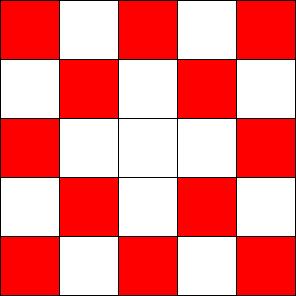
\includegraphics[width=0.15\textwidth]{figures/7/5x5x1.pdf}
\caption{An optimal percolating set for $G(5,5,1)$.}
\label{fig:5x5x1}
\end{figure} 

\begin{figure}[]
\centering
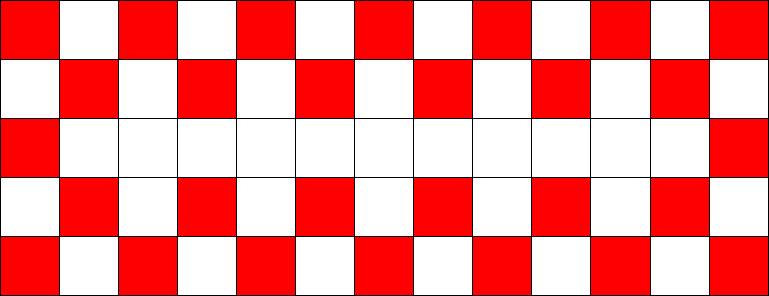
\includegraphics[width=0.5\textwidth]{figures/7/5x13x1.pdf}
\caption{An optimal percolating set for $G(5,13,1)$.}
\label{fig:5x13x1}
\end{figure} 

To extend this construction in the vertical direction, we introduce a ``kink" in the snaking infection. This ``kink" requires six rows to produce a repeating pattern. The structure of this design is shown in Figure \ref{fig:11x13x1}, with the ``kinked" region labeled ``Y". For grids of smaller width, the same construction gives optimal percolating sets; however, the snaking pattern is increasingly difficult to recognize in thin grids.
\end{proof}

\begin{figure}[]
\centering
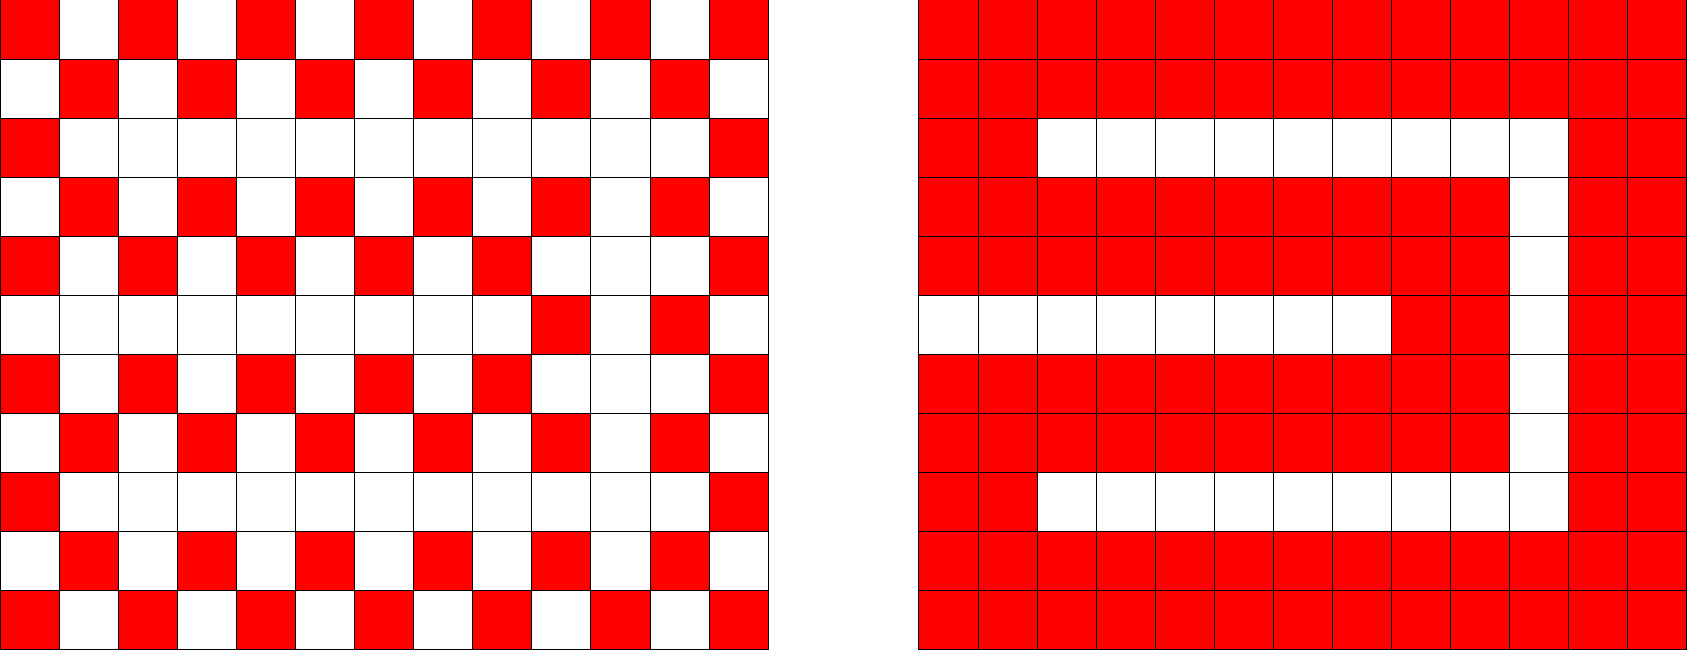
\includegraphics[width=0.6\textwidth]{figures/7/11x13x1.pdf}
\caption{An optimal percolating set for $G(11,13,1)$.}
\label{fig:11x13x1}
\end{figure} 

% Maybe other (divisibility) constructions that percolate at 1 over the bound (if they exist)?

\section{Thickness 2}

We examine four infinite families of grids and show that each admits a lethal set of perfect size. We note that such lethal sets are likely to exist for nearly all divisibility cases in thickness two; however, constructions are elusive and those presented here are sufficient to prove the main result of this thesis.

% (3 mod 6, 3, 2)
\begin{con}
\label{con:3x2x(3mod6)}
All tuples $(a,3,2)$ with $a \equiv 3 \pmod 6$ and $a >3$ are perfect. 
\end{con}

\begin{proof}
%(This construction is the same as the previous one, except the the final four columns are augmented slightly to accommodate the $0 \pmod 3$ requirement. Instead of deriving a proper unfolding, it is probably easier to simply show that this small change is sufficient to guarantee lethality, and agrees with the S.A. bound.)

%We proceed by induction. Consider the grid $G=(9,3,2)$, and let $A_t$ be the set of infected vertices at time-step $t$ (see Figure \ref{fig:9x3x2}). We show that $A_0$ is lethal on $G_1$ and $G_2$. Observe that after one time-step, the subgraph $G_1[\overline{A_1}]$ is a forest connected to the border of $G_1$, and so by Proposition \ref{prop:immune_regions}, $A_0$ is lethal on $G_1$. Since $A_0$ is lethal on $G_1$, by Lemma \ref{lem:2_neighbor_levels}, it is sufficient to prove that $A_0$ is lethal on $G_2$ under the 2-neighbor bootstrap process. Figure \ref{fig:9x3x1} illustrates the key steps of this process, starting at $t=1$. Infection spreads down rows delineated by red arrows, ultimately infecting all vertices in $G_2$. We conclude that $A_0$ is lethal on $G$ under the 3-neighbor process.

%Let $A = \{1\} \times [3] \times [2]$, $B = \{8,9\} \times [3] \times [2]$ and $X = \{2,3,4,5,6,7\} \times [3] \times [2]$ be components of $G$ (see Figure \ref{fig:9x3x2}). Denote by $AX^kB$ the graph obtained by inserting $k$ copies of $X$ between components $A$ and $B$. Let $A_0^k$ be a lethal set on $AX^kB$. We show that $A_0^{k+1}$ is lethal on $AX^{k+1}B$. 

Let $G=G(6k+3,3,2)$ be a grid such that $k>0$. Let $A = \{1\} \times [3] \times [2]$, $B = \{6k+2, 6k+3\} \times [3] \times [2]$, and $X_i = \{6(i-1)+2,6(i-1)+3,\dots,6(i-1)+7\} \times [3] \times [2]$ for $i \in [k]$, be regions of $G$. Denote by $AX^kB$ the union of regions $A \cup X_1 \cup \dots \cup X_{k} \cup B$, and note that $G=AX^kB$. Let $A_t^k \subseteq V(G)$ be the set of infected vertices in $G$ at time $t$, and suppose that each $X_i$ contains the same pattern of infected vertices (see Figure \ref{fig:9x3x2}). We show that the initial infection $A_0^k$ is lethal and perfect.

%Let $G=G(6k+3,3,2)$ be a grid such that $k>0$. Let $A = F_{1,1}$ be the leftmost face of $G$, $B = F_{1,6k+2} \cup F_{1,6k+3}$ be the rightmost two planes of $G$, and $X_i = F_{1,6(i-1)+2} \cup \dots \cup F_{1,6(i-1)+7}$, for $i \in [k]$, be a repeating block of 6 planes of $G$. Denote by $AX^kB$ the union of regions $A \cup X_1 \cup \dots \cup X_{k} \cup B$, and note that $G=AX^kB$. Let $A_t^k \subseteq V(G)$ be the set of infected vertices in $G$ at time $t$, and suppose that each $X_i$ contains the same pattern of infected vertices (see Figure \ref{fig:9x3x2}). We show that the initial infection $A_0^k$ is lethal and perfect. 

Consider the union of regions $AX^k = A \cup X_1 \cup \dots \cup X_{k}$ (see Figure \ref{fig:19x3x2}). Note that this omits the region $B$. Let $L_1$ and $L_2$ be the top and bottom levels of $AX^k$, respectively. Observe that after one time step, the subgraph $L_1[\overline{A_1^k}]$ satisfies the conditions of Proposition \ref{prop:immune_regions}, and so $A_0^k$ is lethal on $L_1$. 

Now consider $AX^kB$ and observe that the top level becomes fully infected (see Figure \ref{fig:21x3x2}). Therefore, by Lemma \ref{lem:2_neighbor_levels}, it is sufficient to prove that $A_0^k$ is lethal on the bottom level under the 2-neighbor bootstrap process. Figure \ref{fig:9x3x1} illustrates the key steps of this process on the smaller grid $AXB$, starting at $t=1$. Infection spreads down rows delineated by red arrows, ultimately infecting all vertices in the bottom level. We conclude that $A_0^k$ is lethal on $G$ under the 3-neighbor process.

To prove that $A_0^k$ is perfect, observe that $|A_0^k| = 3 + 10k + 4$. The surface area bound for $G(6k+3,3,2)$ is given by
$$\frac{(3)(6k+3) + (3)(2) + (2)(6k+3)}{3} = \frac{30k + 21}{3} = 10k+7.$$
Since these two values are equal, $A_0^k$ is tight and lethal, and therefore perfect.
\end{proof}

\begin{figure}[]
\centering
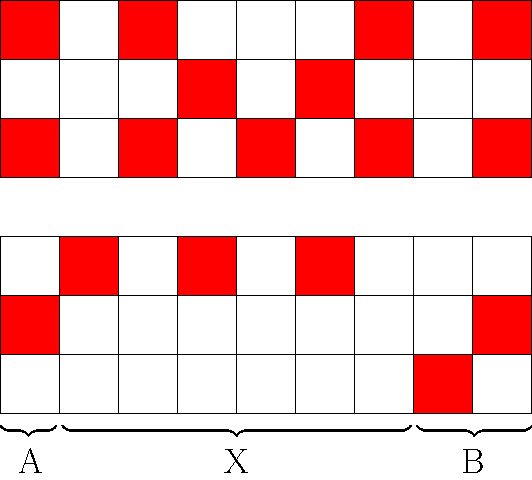
\includegraphics[width=0.3\textwidth]{figures/7/3x9x2.pdf}
\caption{The regions $A$, $X$, $B$ on $G=AXB$ with infectious set $A_0$.}
\label{fig:9x3x2}
\end{figure} 

\begin{figure}[]
\centering
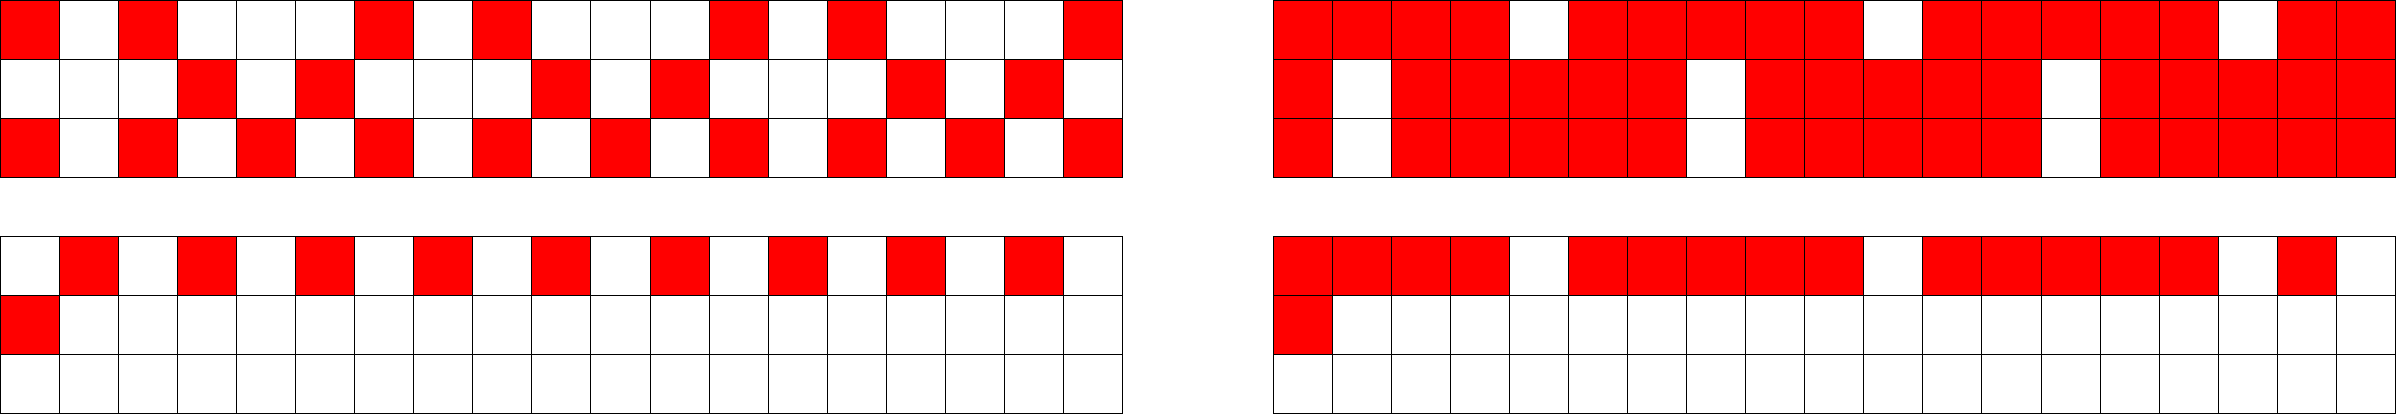
\includegraphics[width=0.8\textwidth]{figures/7/3x19x2.pdf}
\caption{An infection on $AX^3$, $t=0$ and $t=1$.}
\label{fig:19x3x2}
\end{figure} 

\begin{figure}[]
\centering
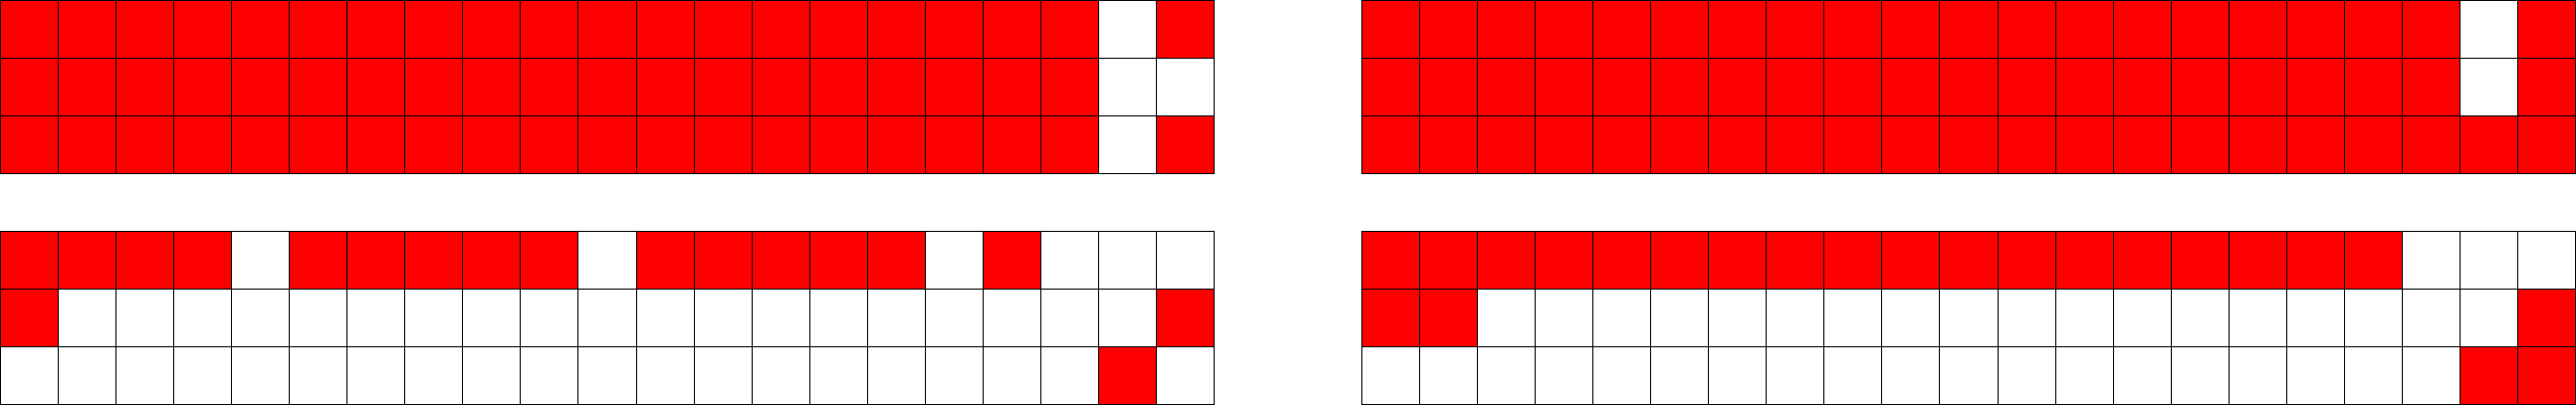
\includegraphics[width=0.8\textwidth]{figures/7/3x21x2.pdf}
\caption{An infection on $G$.}
\label{fig:21x3x2}
\end{figure} 

\begin{figure}[]
\centering
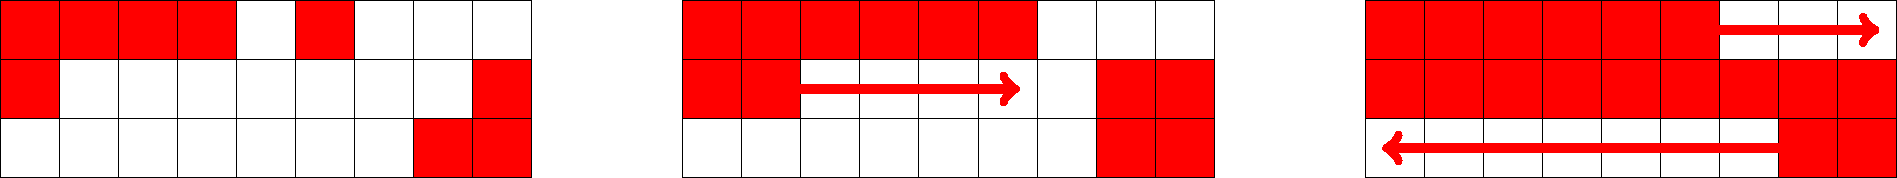
\includegraphics[width=0.8\textwidth]{figures/7/3x9x1.pdf}
\caption{The 2-neighbor process on $G(9,3,1)$ for $t=1$, $2 \le t \le 6$, and $7 \le t \le 14$.}
\label{fig:9x3x1}
\end{figure} 

\begin{con}
\label{con:3x2xa_mod6}
All tuples $(a,3,2)$ with $a \equiv 0 \pmod 6$ and $a \geq 6$ are perfect. 
\end{con}

\begin{proof}
Let $G=G(a,3,2)$ where $a \equiv 0 \pmod 6$ and $a \geq 6$, and let $M$ be the manifold of $G$ illustrated in Figure \ref{fig:3x12x2_manifold_a} and $H$ be its proper unfolding (see Figure \ref{fig:3x12x2_manifold_b}). Observe that $M$ is indeed a manifold: it partitions $V(G) \setminus M$ into two sets $R_1$ and $R_2$, both bounded by mutually orthogonal red, green, and blue faces (see Figure \ref{fig:3x12x2_manifold_a}). Furthermore, note that $H$ is obtained from $M$ by cutting along seams between red and green faces, and flattening the figure. It follows that $H$ is a proper unfolding of $G$. 

Let $X_1, \dots, X_k$ be the periodic regions of $H$ of width $6$ (see Figure \ref{fig:3x12x2_unfolded_lethal}). Denote by $X^k$ the union of these regions. Let $A_0$ be a set of initially infected vertices in $H$ and $A_t \subseteq V(H)$ be the set of infected vertices in $H$ at time $t$. Note that each $X_i$, for $i \in [k]$, contains the same pattern of infected vertices (see Figure \ref{fig:3x12x2_unfolded_lethal}). We show that $A_0$ is lethal and perfect.

Figure \ref{fig:3x12x2_unfolded_lethal} shows $A_0$ in $H$. Observe that $A_0$ infects all vertices of $X^k$ by Proposition \ref{prop:immune_regions}. We show that the remaining healthy vertices of $H$ become infected. Consider re-folding $H$, and note that both pairs of cells marked with an ``X" in $H$ represent the same cell in $G$. This is enough to infect the remaining regions of $H$, and by Corollary \ref{cor:three_walls}, $A_0$ is lethal on $G$. 
%Furthermore, observe that $G$ can be extended in the $x$ direction by repeated insertions of the component $X$ (see Figure \ref{fig:3x12x2}). This process does not affect the structure of $H$, and Proposition \ref{prop:immune_regions} again guarantees lethality.

To prove that $A_0$ is perfect, observe that $|A_0| = 4 + 10k + 8 = 10k +12$. The surface area bound for $G(6k+6,3,2)$, where $k$ is the number of repeated regions $X$, is given by
$$\frac{(3)(6k+6) + (3)(2) + (2)(6k+6)}{3} = \frac{30k + 36}{3} = 10k+12.$$
Since these two values are equal, $A_0$ is tight and lethal, and therefore perfect.
\end{proof}

% (0 mod 6, 3, 2)

\begin{figure}[]
\centering
\begin{subfigure}{0.45\textwidth}
	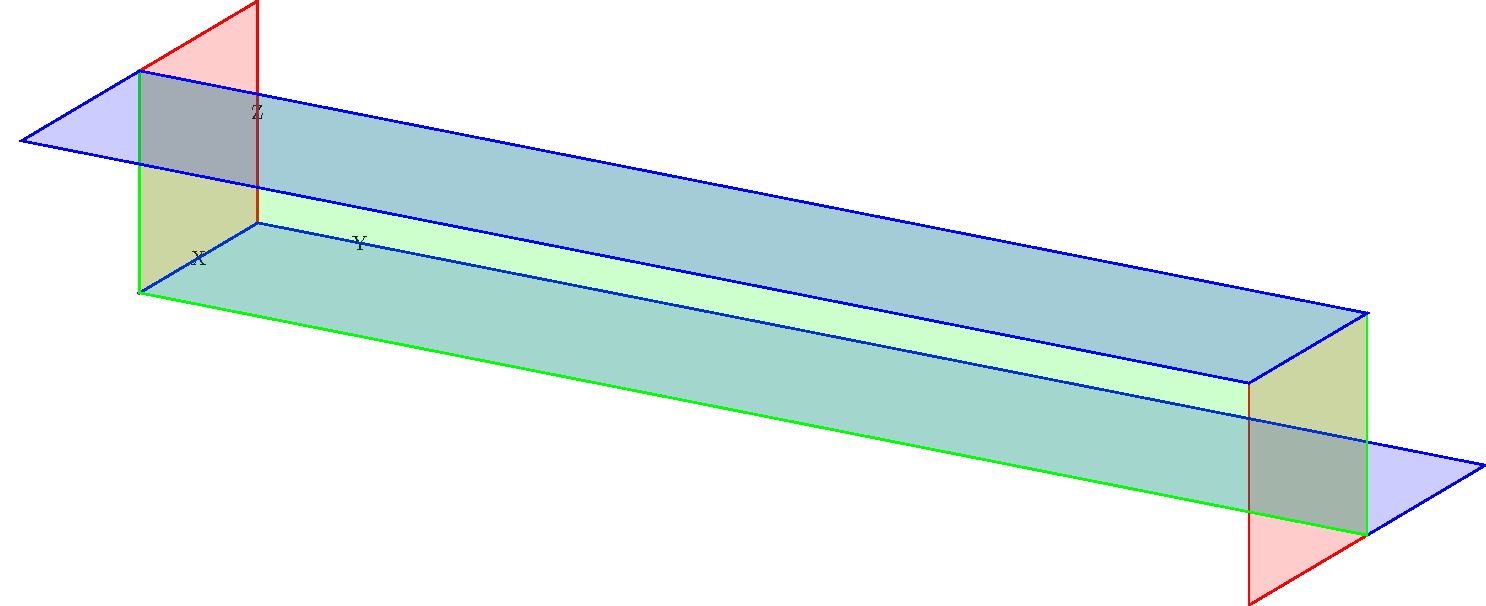
\includegraphics[width=\textwidth]{figures/7/3x12x2_manifold_3d.pdf}
	\caption{A manifold of $G(3,12,2)$.}
	\label{fig:3x12x2_manifold_a}
\end{subfigure} \hfill%
\begin{subfigure}{0.45\textwidth}
	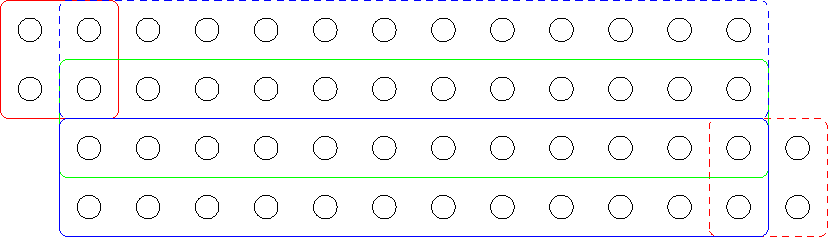
\includegraphics[width=\textwidth]{figures/7/3x12x2_manifold.pdf}
	\caption{A proper unfolding of $G$.}
	\label{fig:3x12x2_manifold_b}
\end{subfigure}
\caption{A proper unfolding of $G(3,12,2)$. Colored rectangles indicate faces of $G$. Dashed lines indicate that cells appear on different layers. }
\label{fig:3x12x2_manifold}
\end{figure} 

\begin{figure}[]
\centering
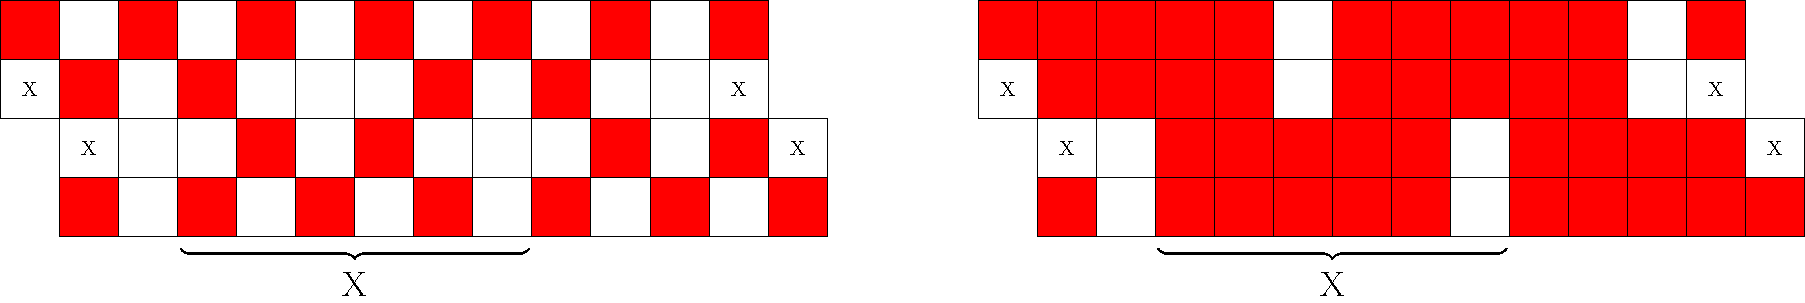
\includegraphics[width=0.8\textwidth]{figures/7/3x12x2_unfolded_lethal.pdf}
\caption{A lethal set on $H$ showing the repeated region $X$ ($t=1$ and $t=2$).}
\label{fig:3x12x2_unfolded_lethal}
\end{figure} 

\begin{figure}[]
\centering
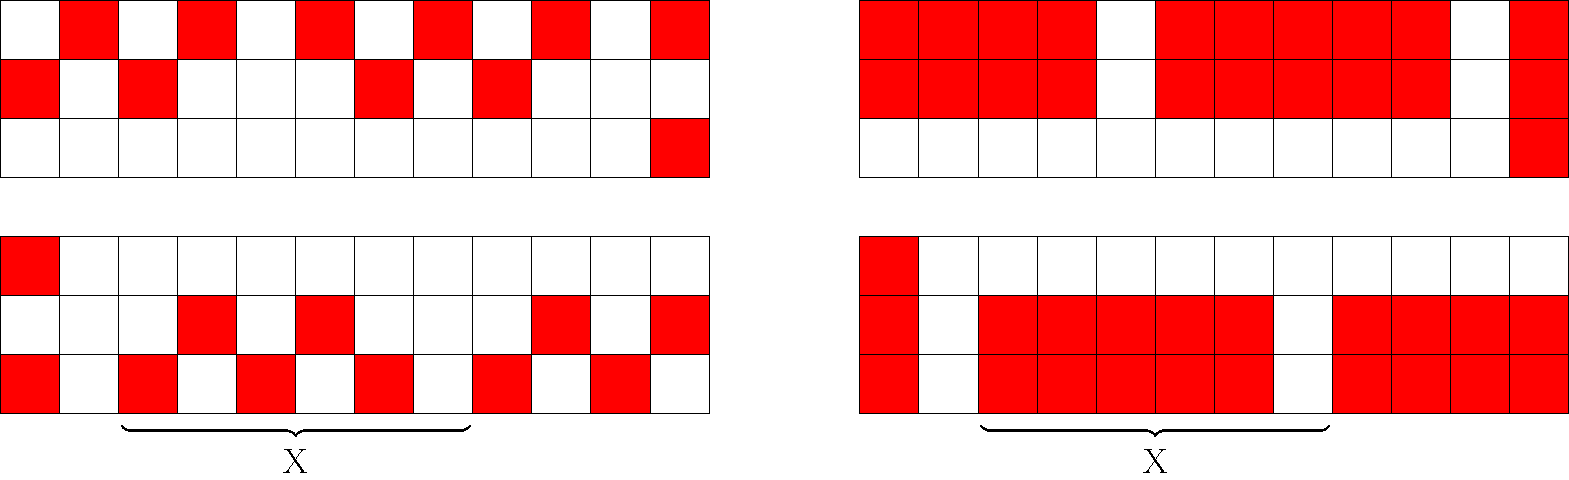
\includegraphics[width=0.8\textwidth]{figures/7/3x12x2.pdf}
\caption{A perfect lethal set for $G(3,12,2)$ with region $X$.}
\label{fig:3x12x2}
\end{figure} 

% (2 mod 6, 5 mod 6, 2)

% a,b, MUST BE A CERTAIN SIZE
\begin{con}
\label{con:2x2x5_mod6}
All tuples $(a,b,2)$ with $a,b \in \{2,5\} \pmod 6$, $a \not\equiv b \pmod 6$, and $a,b > 2$ are perfect. 
\end{con}

\begin{proof}
Let $G=G(a,b,2)$ be a grid with $a,b \in \{2,5\} \pmod 6$, $a \not\equiv b \pmod 6$, and $a,b > 2$, and let $M$ be a manifold of $G$ and $H$ be its proper unfolding (Figure \ref{fig:11x20x2_manifold}). Note that $M$ partitions the vertices of $V(G) \setminus M$ into two disjoint sets $R_1$ and $R_2$, both bounded by mutually orthogonal red, green, and blue faces. Note, also, that $H$ is obtained from $M$ by cutting along seams between red and green faces, and flattening the figure. Therefore, $H$ is a proper unfolding of $G$. 

Let $X_1, \dots, X_{k_1}$ be the repeated regions of $H$ in the $x$-direction, and $Y_1, \dots, Y_{k_2}$ be the repeated regions of $H$ in the $y$-direction (see Figure \ref{fig:18x16x1_unfolded_lethal}). Denote by $X_iY_j$ the region obtained from $X_i \cap Y_j$, and let $X^{k_1}Y^{k_2}$ be the union of all $X_iY_j$. Let $A_t \subseteq V(H)$ be the set of infectious vertices in $H$ at time $t$, and suppose that for $i \in [k_1] \setminus \{1,k_1\}$ and $j \in [k_2]$, each $X_iY_j$ contains the same pattern of infected vertices (see Figure \ref{fig:XiYj}). We show that $A_0$ is lethal and perfect.

Consider the initial infection $A_0$ of $H$ as shown in Figure \ref{fig:18x16x1_unfolded_lethal}. Observe that $A_0$ infects all vertices of $X\times Y$ by Proposition \ref{prop:immune_regions}. We show that the remaining healthy vertices of $H$ become infected. The individual vertices in the rightmost column of $H$ are infected by Proposition \ref{prop:immune_regions}. Consider re-folding $H$, and note that the pairs of cells marked with an ``X" in $H$ represent the same cell in $G$. This is enough to infect the remaining regions of $H$, and by Corollary \ref{cor:three_walls}, $A_0$ is lethal on $G$. 

To prove that $A_0$ is perfect, observe that for $i \in [k_1] \setminus \{1\}$ and $j \in [k_2]$, each $X_iY_j$ block contains exactly 12 infected vertices. For $j \in [k_2 -1]$, $X_1Y_j$ contains 11 infected vertices, and $X_1Y_{k_2}$ contains 12 infected vertices. In total, the region $XY$ contains exactly 
$$12(k_1-1)(k_2) + 11(k_2-1) + 12$$
initially infected vertices. Of the remaining vertices in $H$, $14k_1 - 1 +9k_2 + 8$ are infected. Therefore, 
\begin{align*}
|A_0| &= 12(k_1-1)k_2 + 11(k_2-1) + 12+14(k_1) - 1 +9(k_2) + 8 \\
&= 12k_1k_2 + 14k_1 + 8k_2 +8.
\end{align*}
The surface area bound for $G(6k_1+2,6k_2+5,2)$ is given by
\begin{align*}
SA(6k_1+2,6k_2+5,2) &= \frac{(6k_1+2)(6k_2 + 5) + (6k_2+5)(2) + (2)(6k_1+2)}{3} \\
&= \frac{36(k_1)(k_2) +42k_1 +24k_2 + 24}{3} \\
&= 12k_1k_2 +14k_1+8k_2+8.
\end{align*}
Since these two values are equal, $A_0$ is tight and lethal, and therefore perfect.
\end{proof}

\begin{figure}[]
\centering
\begin{subfigure}{0.45\textwidth}
	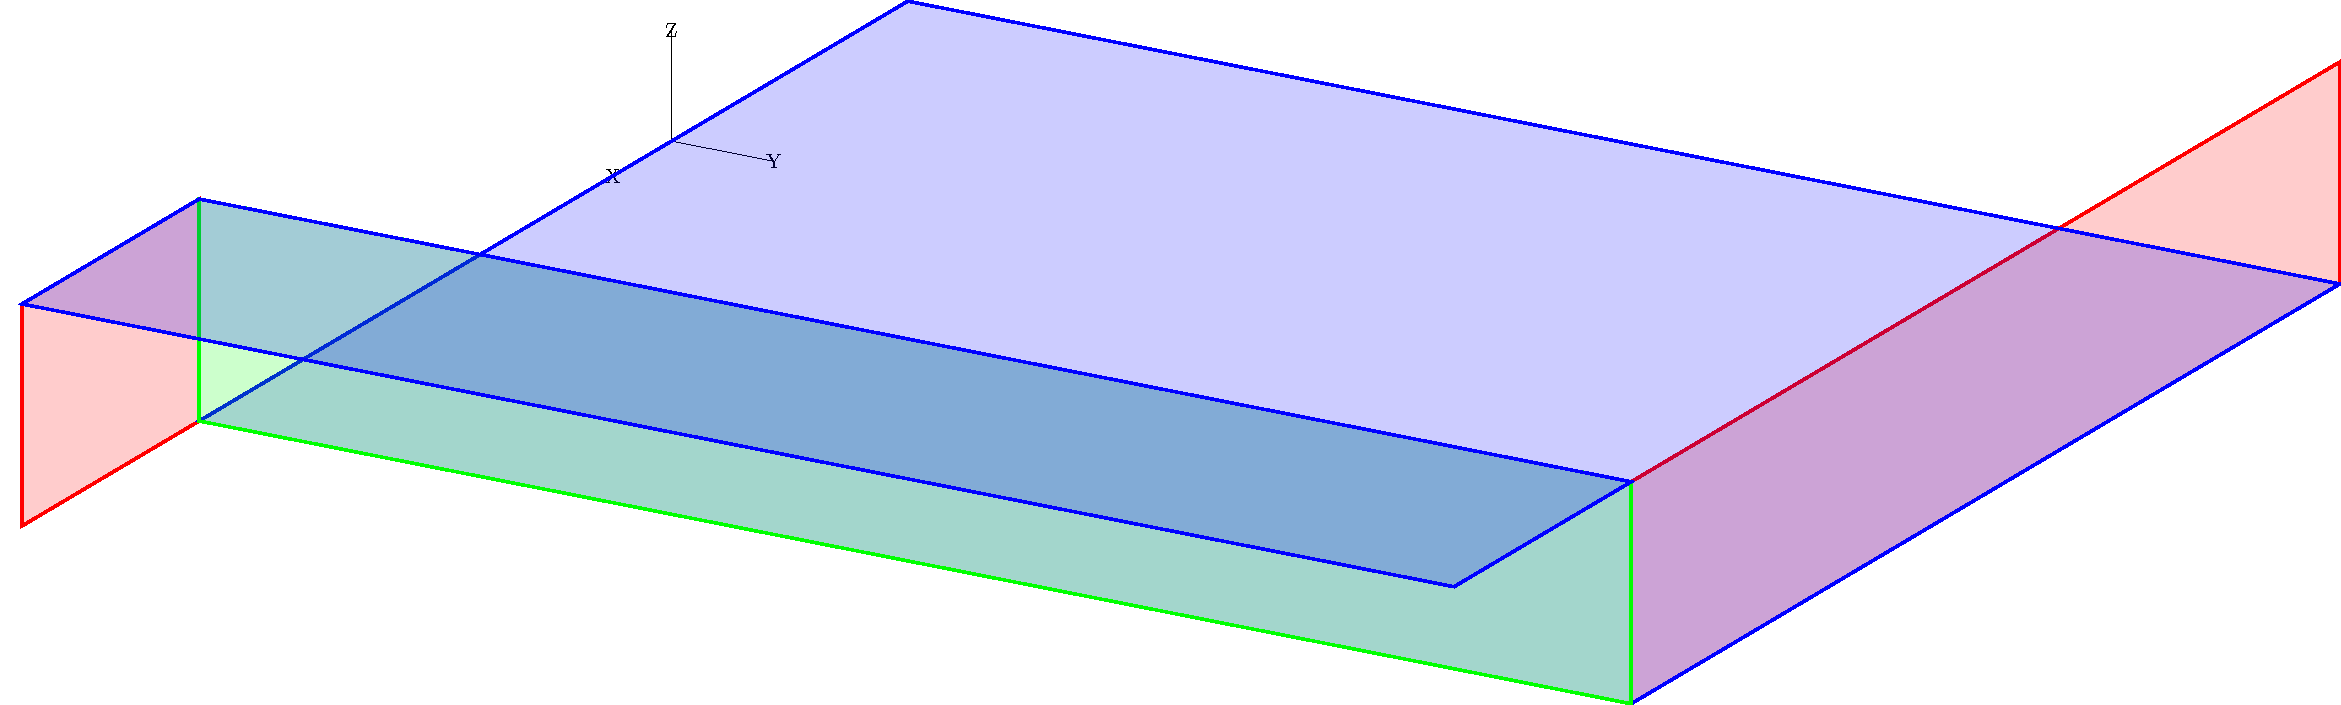
\includegraphics[width=\textwidth]{figures/7/11x20x2_manifold_3d.pdf}
	\caption{A manifold of $G(11,20,2)$.}
	\label{}
\end{subfigure} \hfill%
\begin{subfigure}{0.45\textwidth}
	
\includegraphics[width=\textwidth]{figures/7/11x20x2_manifold.pdf}
	\caption{A proper unfolding of $G$.}
	\label{}
\end{subfigure}
\caption{A proper unfolding of $G(11,20,2)$. Colored rectangles indicate faces of $G$. Dashed lines indicate that cells appear on different layers. }
\label{fig:11x20x2_manifold}
\end{figure} 

\begin{figure}[]
\centering
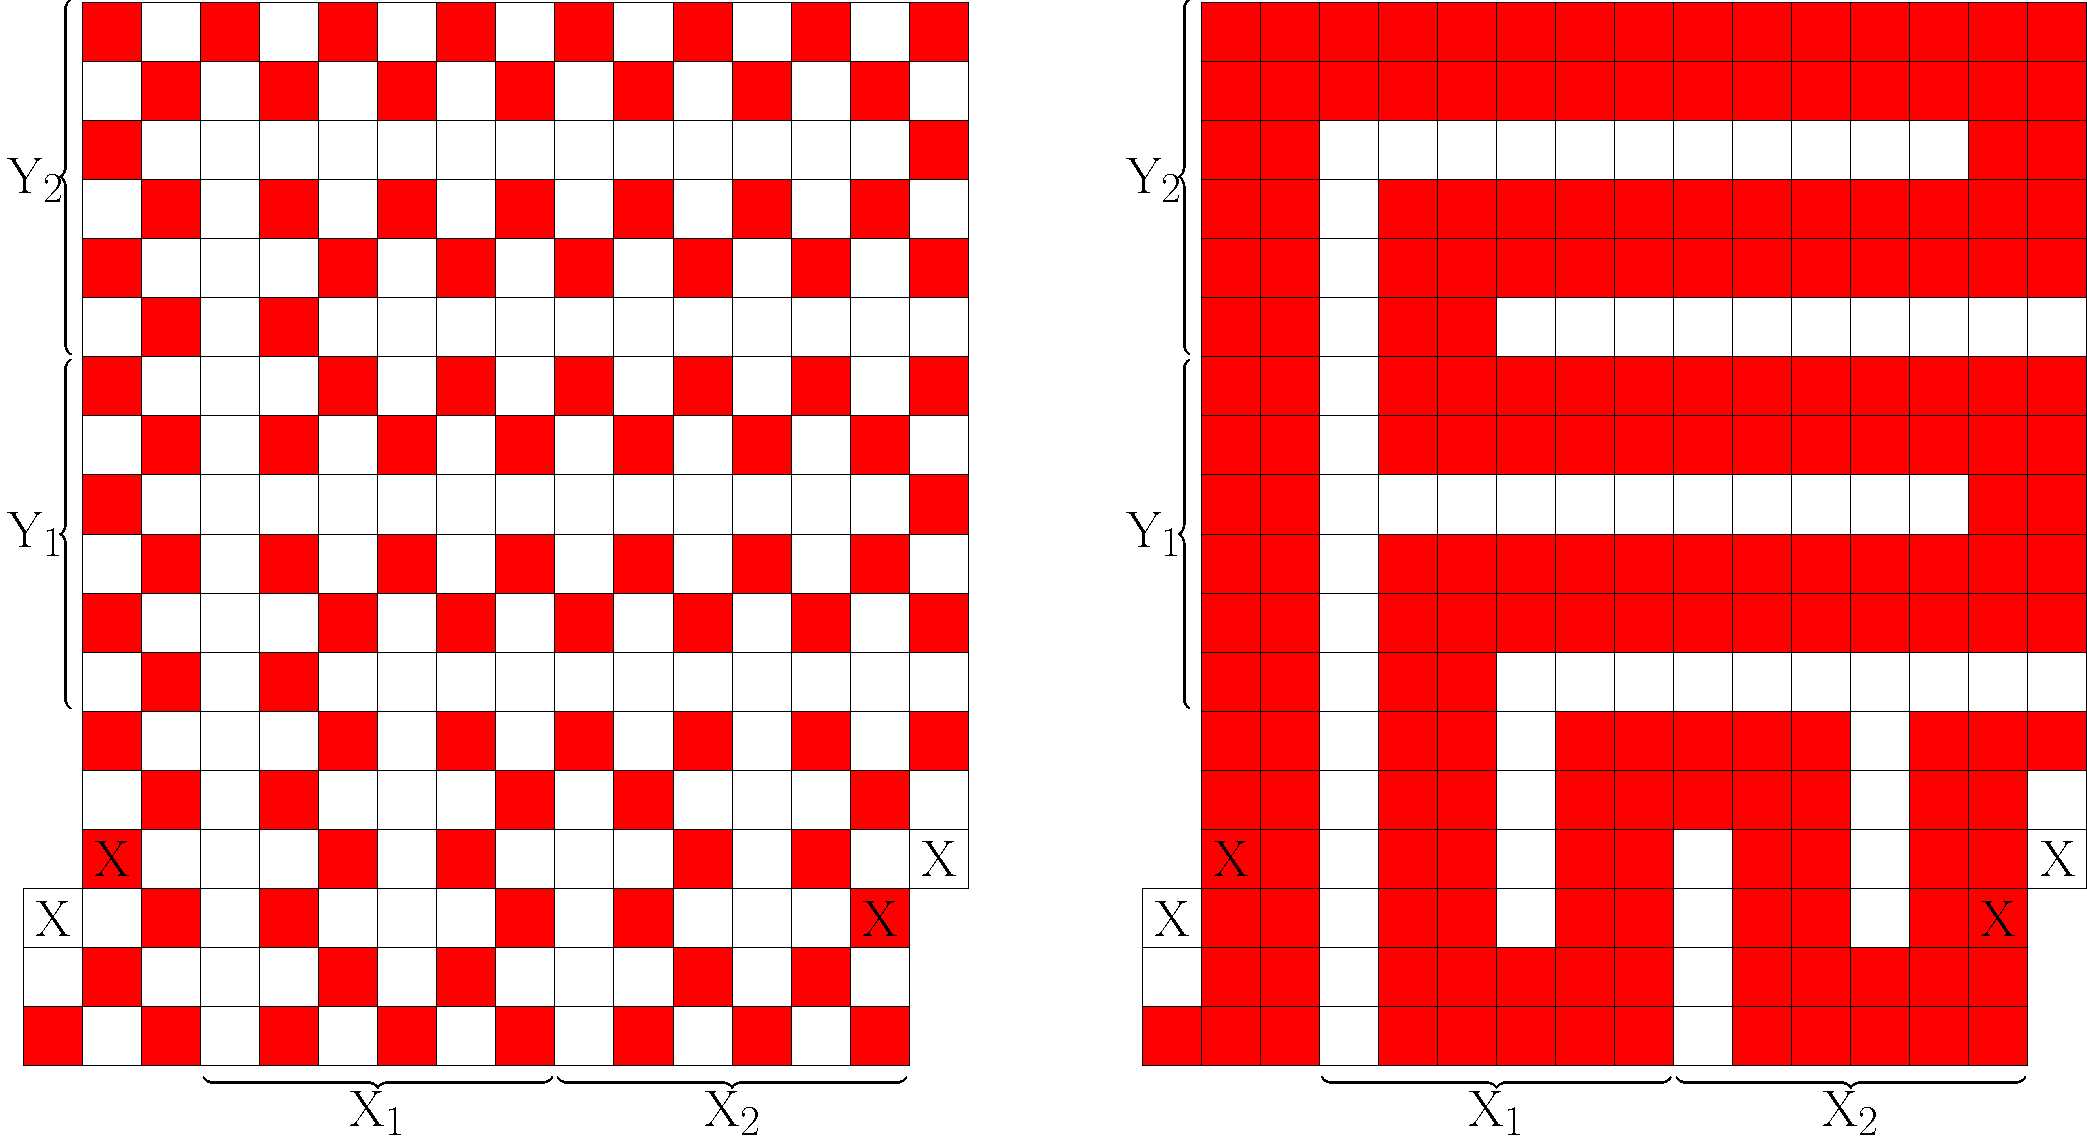
\includegraphics[width=0.8\textwidth]{figures/7/18x16x1_unfolded_lethal.pdf}
\caption{A percolating set on the proper unfolding of $G(17,14,2)$.}
\label{fig:18x16x1_unfolded_lethal}
\end{figure}

\begin{figure}[]
\centering
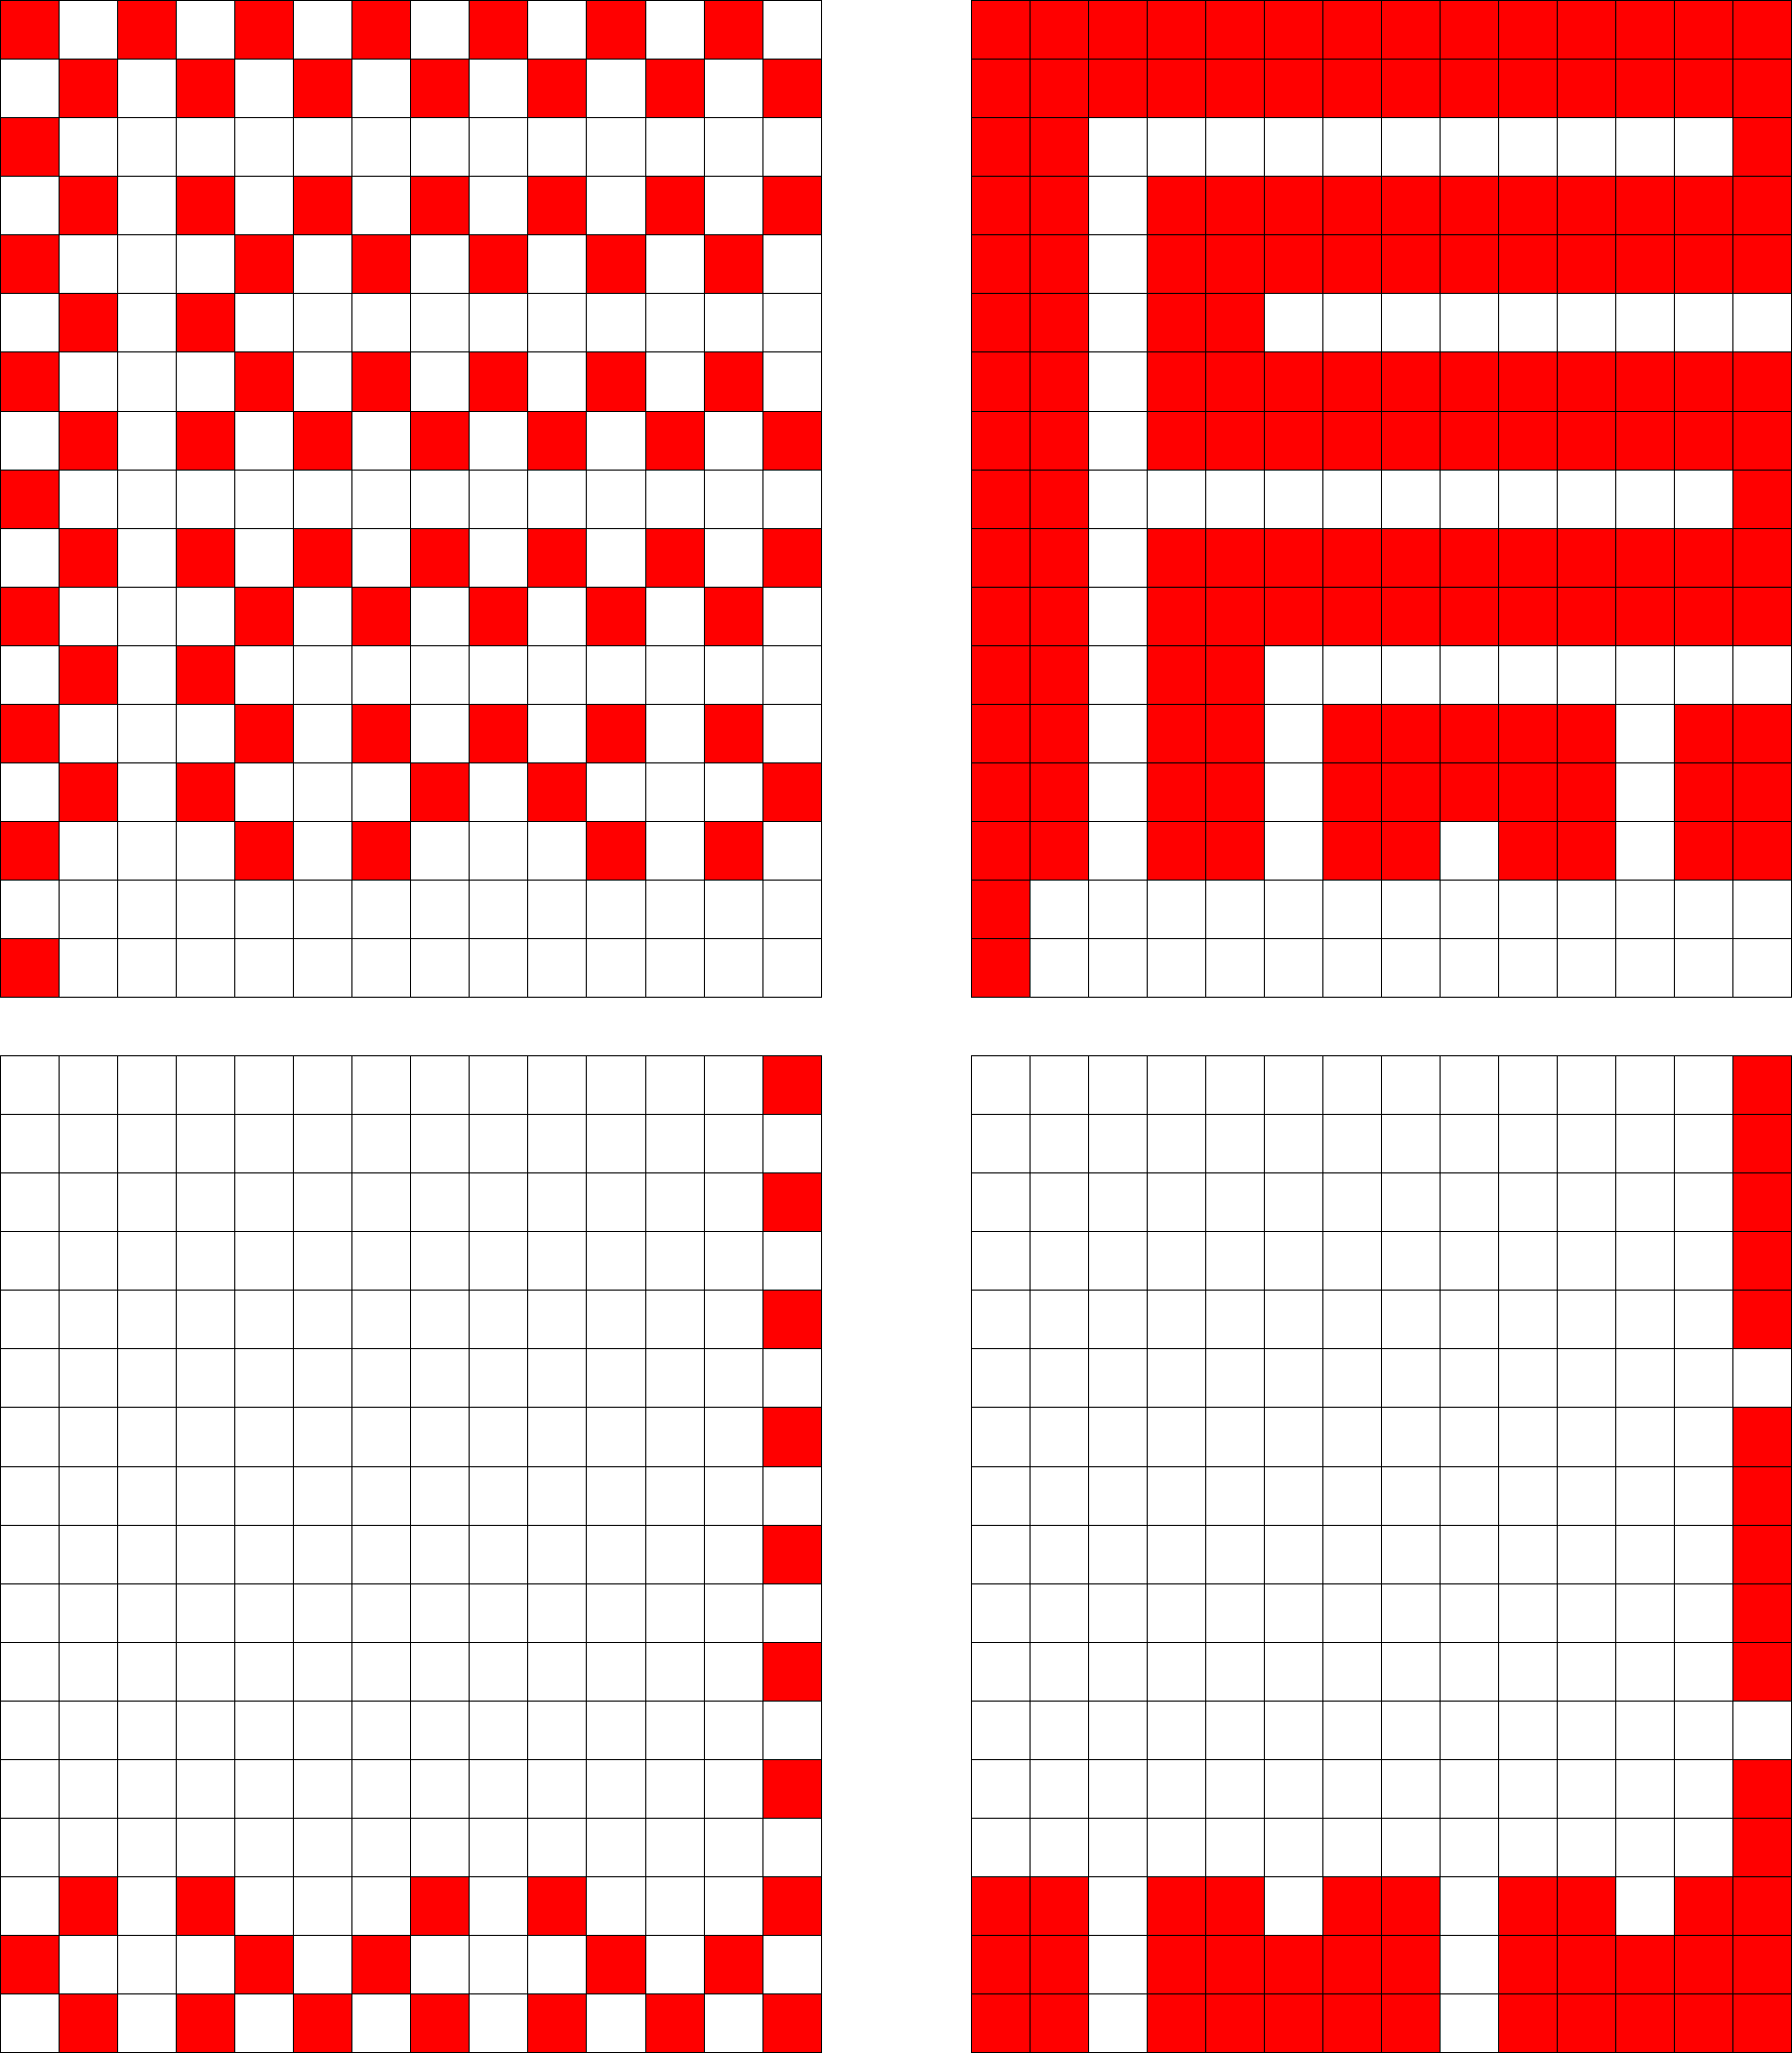
\includegraphics[width=0.6\textwidth]{figures/7/17x14x2.pdf}
\caption{A perfect percolating set for $G(17,20,2)$.}
\label{fig:11x20x2}
\end{figure} 

\begin{figure}[]
\centering
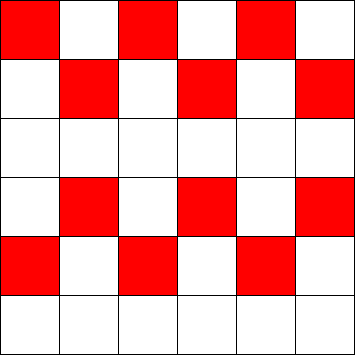
\includegraphics[width=0.12\textwidth]{figures/7/XiYj.pdf}
\caption{A block $X_iY_j$.}
\label{fig:XiYj}
\end{figure} 

% (3 mod 6, 0 mod 6, 2) 

% a,b MUST BE A CERTAIN SIZE
\begin{con}
\label{con:2x3x0_mod6}
All tuples $(a,b,2)$ with $a,b \in \{0,3\} \pmod 6$, $a \not\equiv b \pmod 6$ and $a,b, \geq 6$ are perfect. 
\end{con}

\begin{proof}
Let $G=G(a,b,2)$ be a grid with $a,b \in \{0,3\} \pmod 6$, $a \not\equiv b \pmod 6$, and $a,b \geq 6$, and let $X_1, \dots, X_{k_1}$ be the repeated regions of $G$ in the $x$-direction, and $Y_1, \dots, Y_{k_2}$ be the repeated regions of $G$ in the $y$-direction (see Figure \ref{fig:12x15x2}). Denote by $X_iY_j$ the region obtained from $X_i \cap Y_j$, and let $X^{k_1}Y^{k_2}$ be the union of all $X_iY_j$. Let $A_t \subseteq V(H)$ be the set of infected vertices in $G$ at time $t$, and suppose that for $i \in [k_1]$ and $j \in [k_2]$, each $X_iY_j$ contains the same pattern of infected vertices (see Figure \ref{fig:12x15x2}). We show that $A_0$ is lethal and perfect.

Let $L_1$ and $L_2$ be the top and bottom layers of $G$, respectively. Observe that after one time step, the subgraph of $L_1$ induced by the uninfected vertices of $\cup Y_i$ is both acyclic and contains no border-to-border paths. Therefore, by Proposition \ref{prop:immune_regions}, $A_0$ is lethal in $(\cup Y_i) \cap L_1$. 

Consider these observations in the context of $G$. Figure \ref{fig:12x15x2_L1} shows that after 5 additional time-steps, the remaining healthy vertices in $L_1$ form two paths, marked by red arrows. The vertices in the upper path are infected by Proposition \ref{prop:immune_regions}, and those in the lower path are infected by Lemma \ref{lem:2_neighbor_levels}. Therefore, all vertices of $L_1$ become infected. Furthermore, the infected vertices in $L_2$ form a lethal set under the 2-neighbor process, and so, by Lemma \ref{lem:2_neighbor_levels}, we conclude that $A_0$ is lethal on $G$ under the 3-neighbor process.

To prove that $A_0$ is perfect, observe that for $i \in [k_1]$ and $j \in [k_2]$, each $X_iY_j$ block contains exactly 12 infected vertices, and so the total number of infected vertices in $XY$ is $12k_1k_2$. 

Of the remaining vertices in $G$, $16k_1+22k_2+28$ are infected. Therefore,
$$|A_0| = 12k_1k_2 + 16k_1+22k_2+28.$$ 
The surface area bound for $G(6k_1+9,6k_2+6,2)$ is given by
\begin{align*}
SA(6k_1+9,6k_2+6,2) &= \frac{(6k_1+9)(6k_2+6) + (6k_2+6)(2) + (2)(6k_1+9)}{3} \\
&= \frac{36k_1k_2+ 48k_1 + 66k_2 + 84}{3} \\
&= 12k_1k_2+16k_1+22k_2+28.
\end{align*}
Since these two values are equal, $A_0$ is tight and lethal, and therefore perfect.
\end{proof}

\begin{figure}[]
\centering
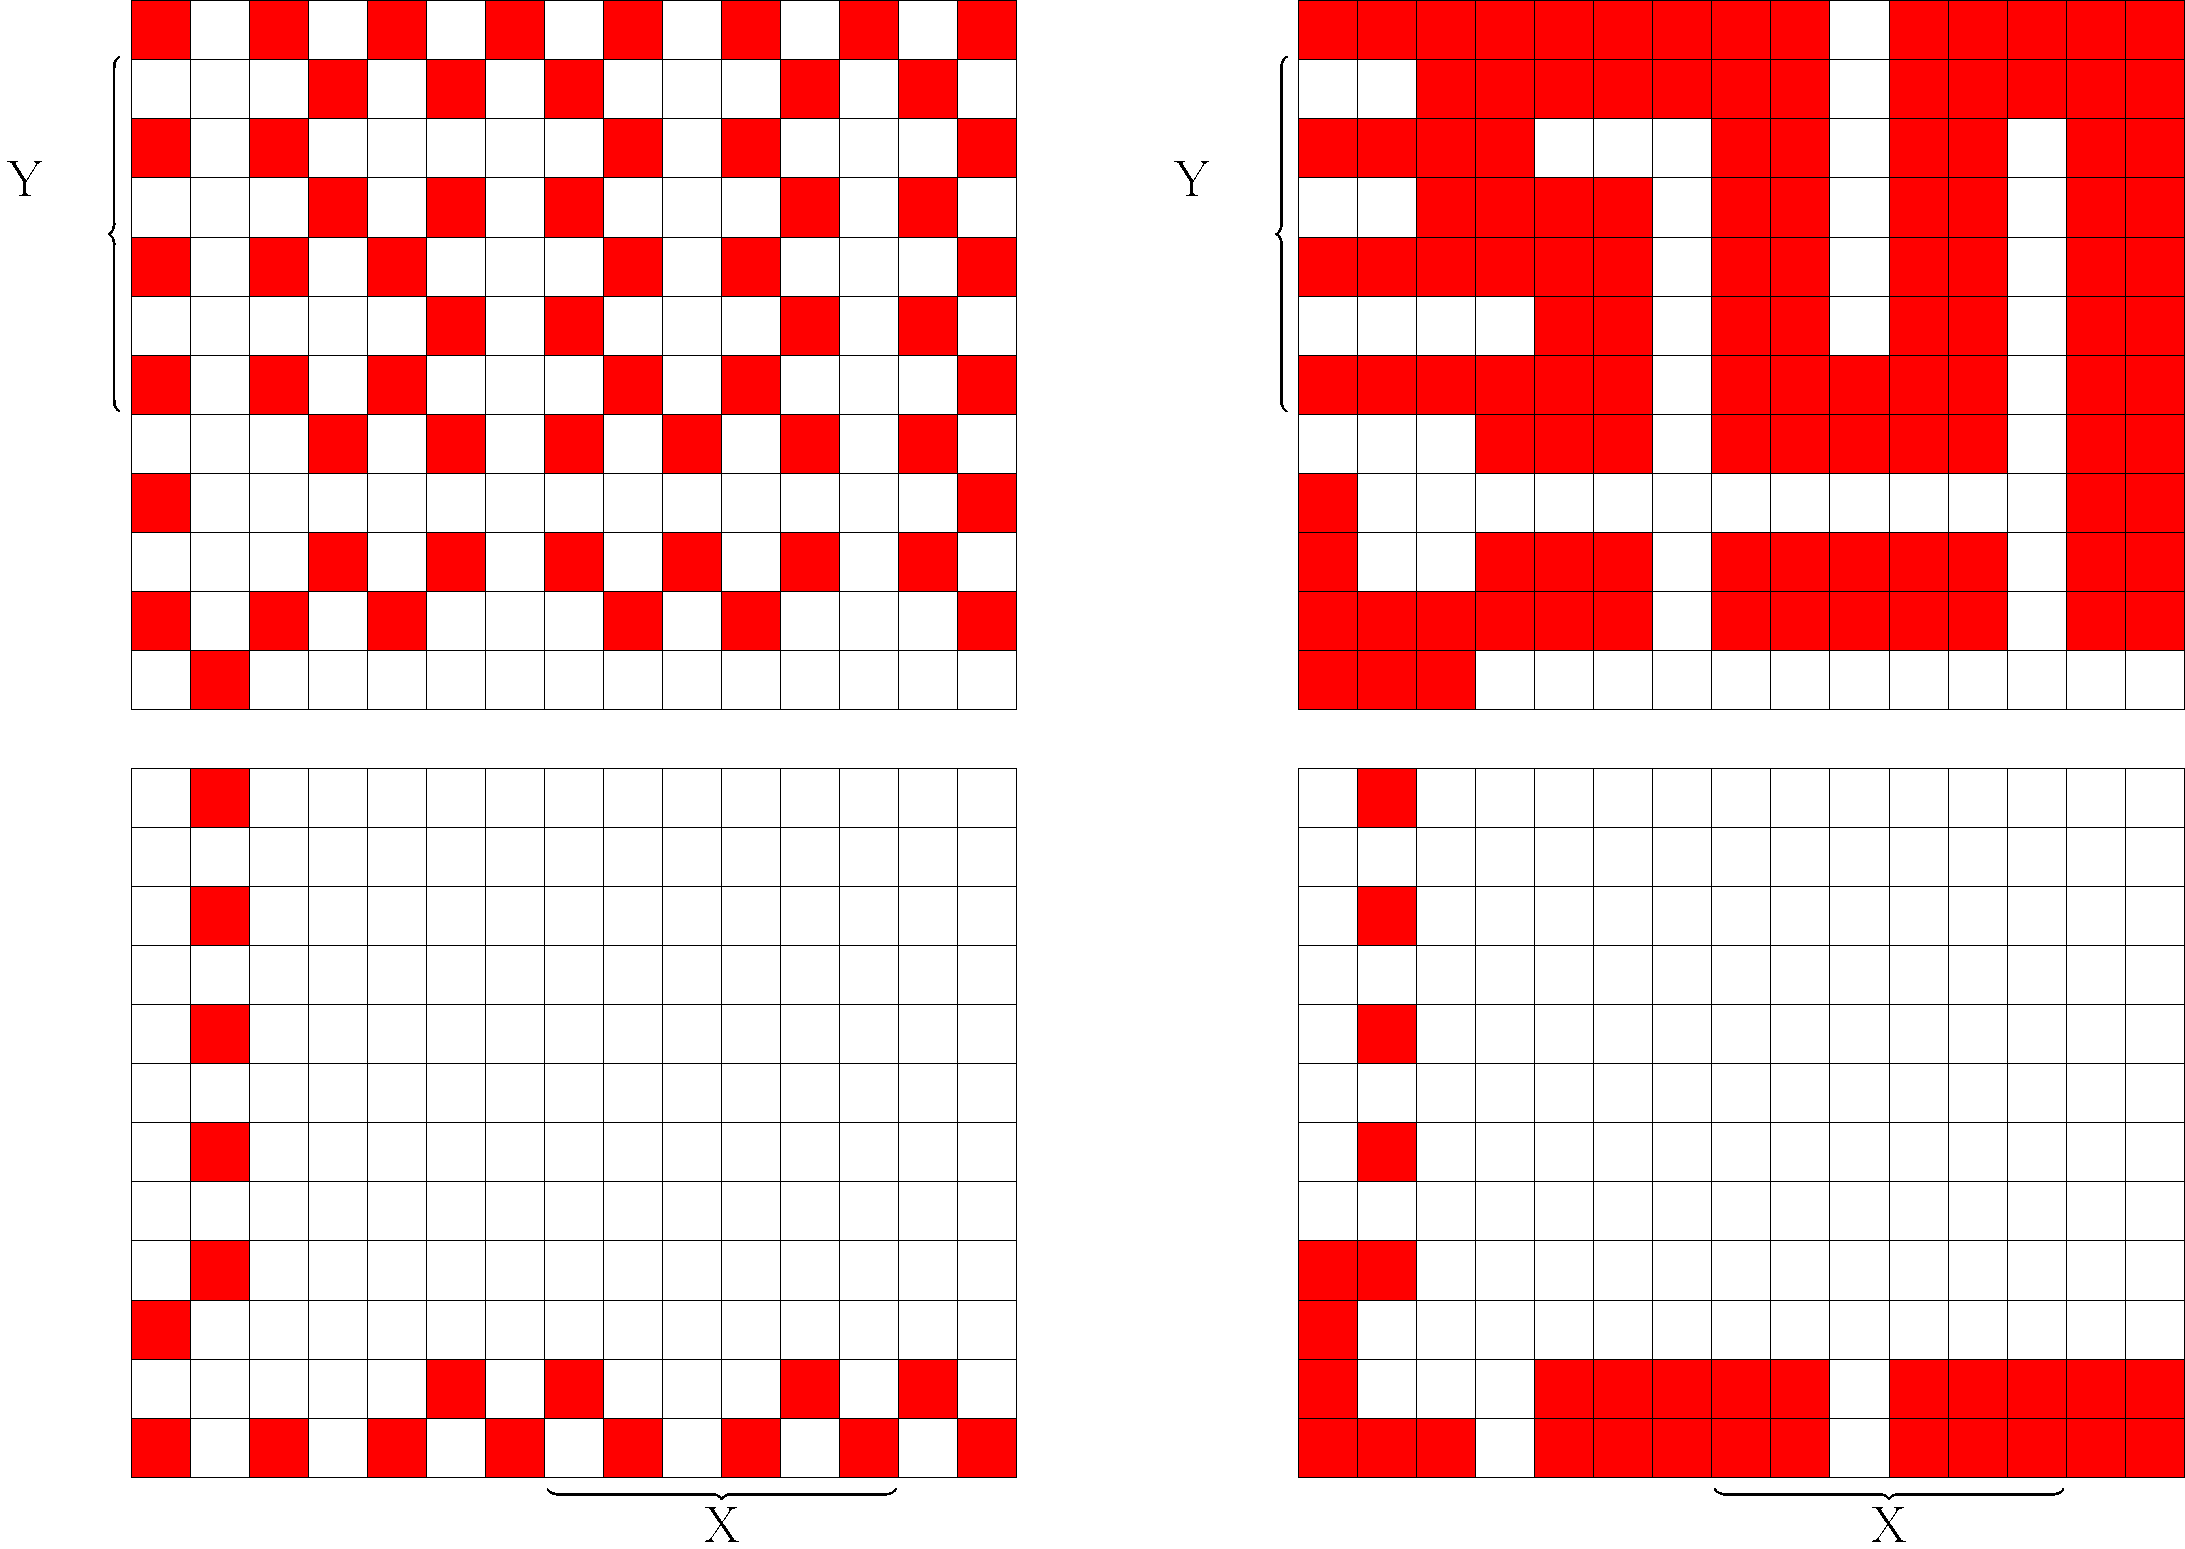
\includegraphics[width=0.8\textwidth]{figures/7/12x15x2.pdf}
\caption{A perfect percolating set for $G(12,21,2)$.}
\label{fig:12x15x2}
\end{figure} 

\begin{figure}[]
\centering
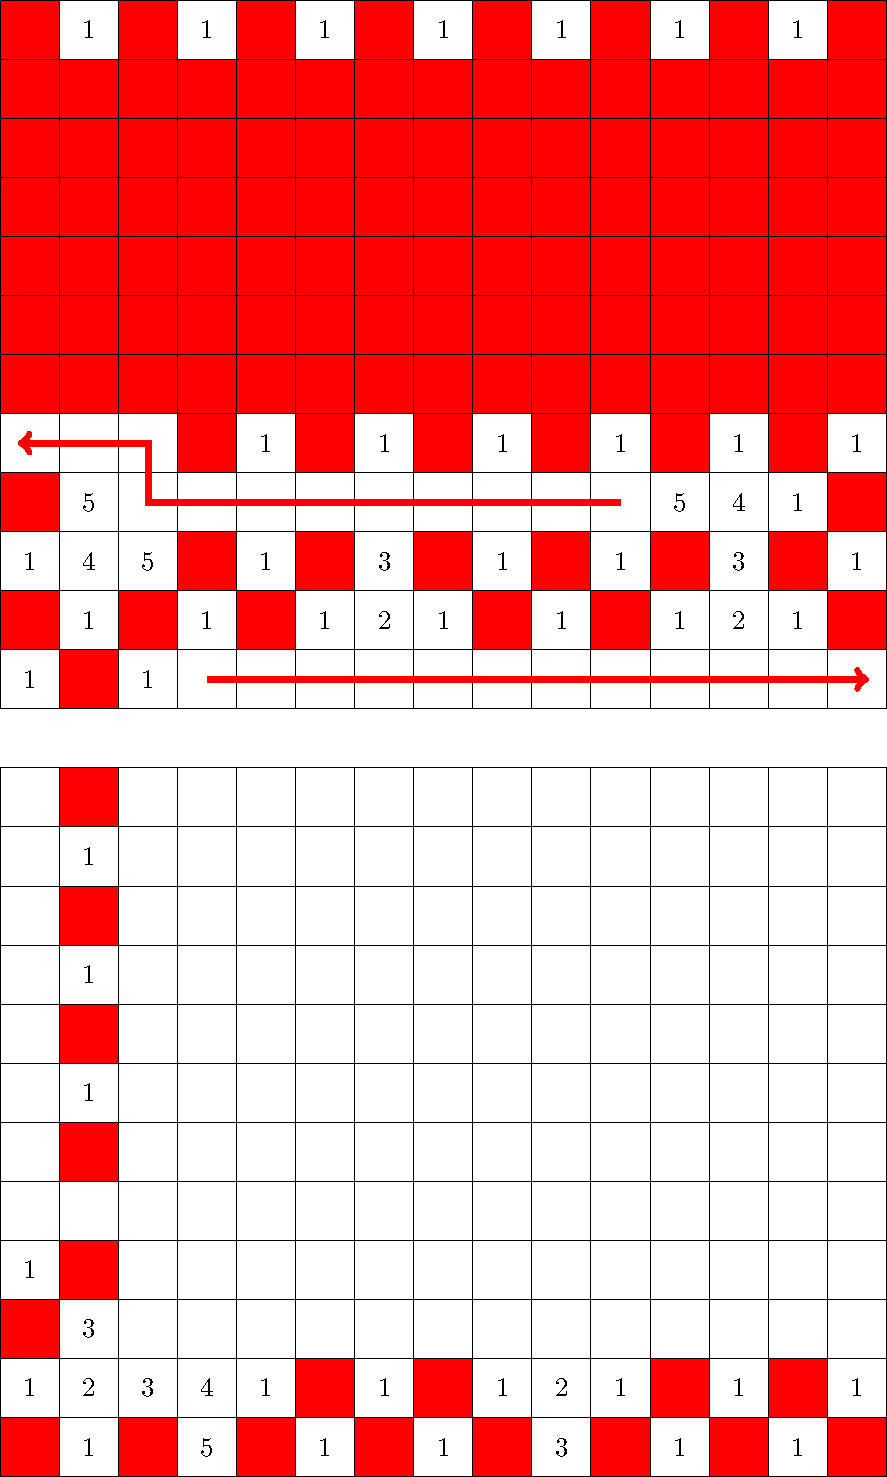
\includegraphics[width=0.6\textwidth]{figures/7/12x15x2_L1_numbered_heatmap.pdf}
\caption{Time steps of infection from a perfect lethal set on $G(12,21,2)$.}
\label{fig:12x15x2_L1}
\end{figure} 

We note that it is possible to examine grids of the form described above using a folding argument, \emph{if} they are at least as large as $G(12,21,2)$. However, such a process omits an infinite number of smaller grids. Nevertheless, the construction contributes to the set of possible shapes of manifold, and the grid and corresponding unfolded net are given in Figures \ref{fig:12x21x2}, \ref{fig:12x21x2_unfolded} and \ref{fig:12x21x2_unfolded_lethal} in the Appendix. 

% COMMENT
% COMMENT
% COMMENT
\begin{comment}

\begin{figure}[]
\centering
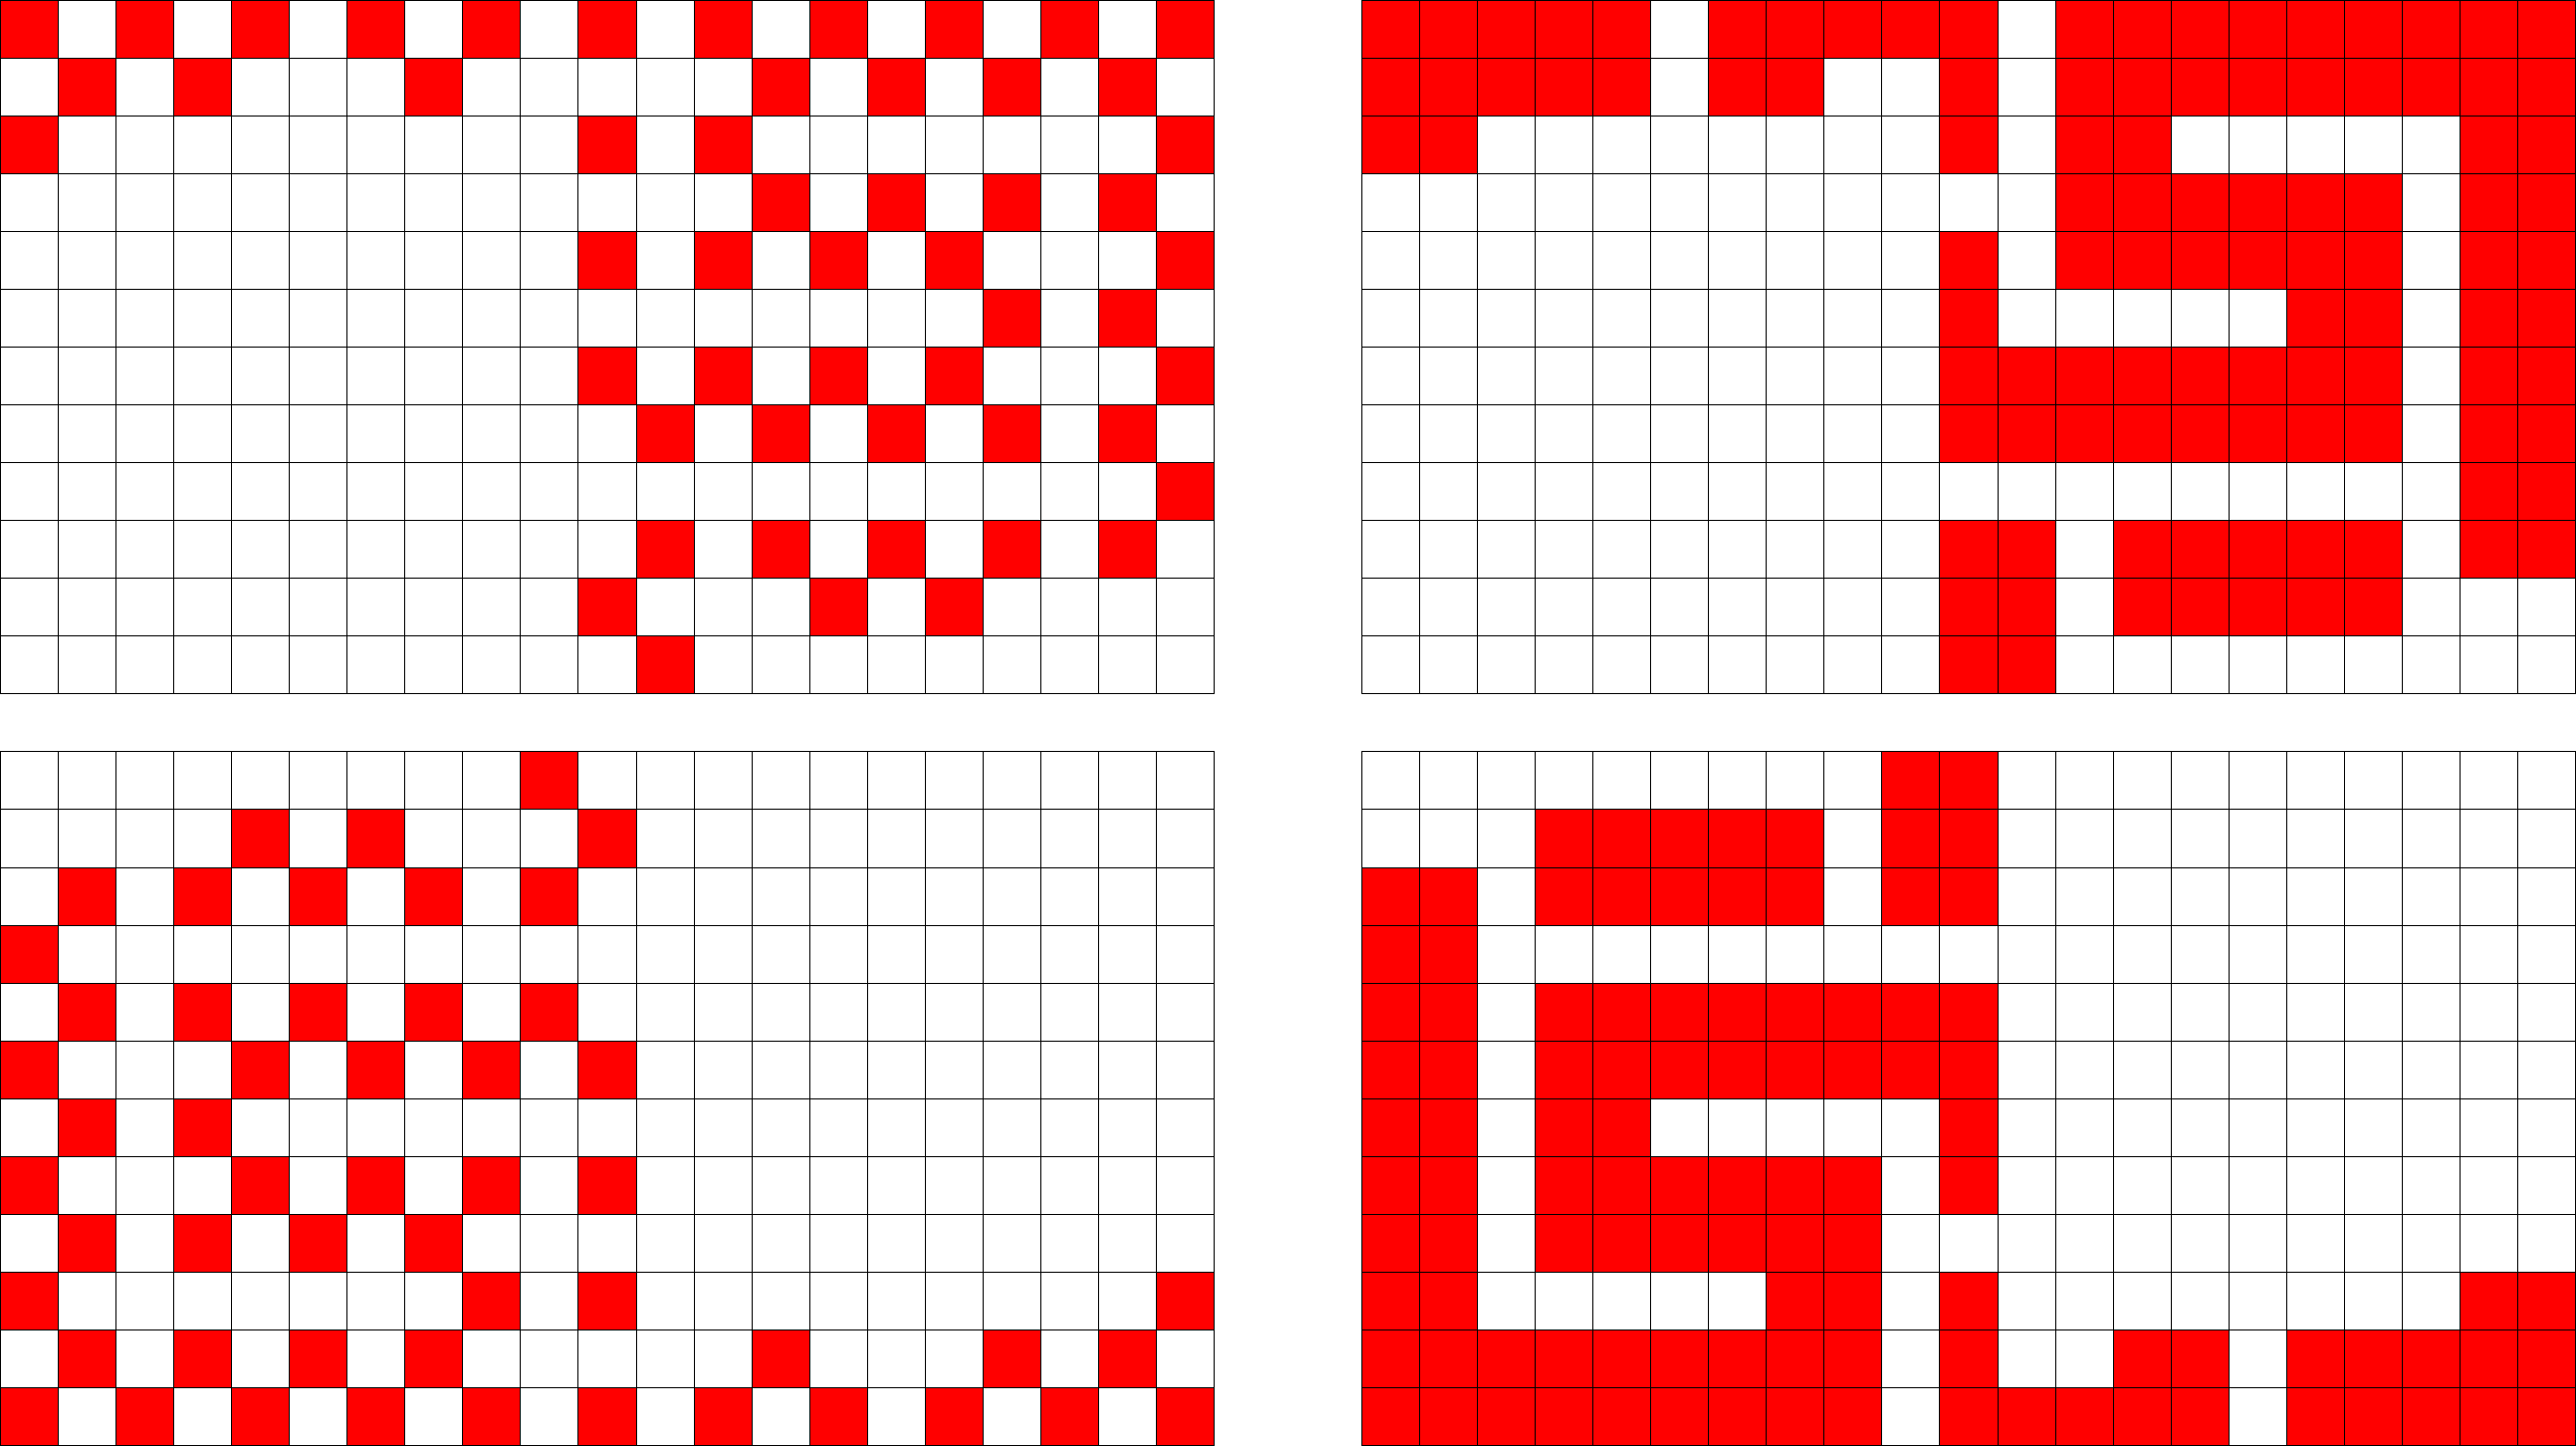
\includegraphics[width=0.8\textwidth]{figures/7/12x21x2.pdf}
\caption{A perfect percolating set for $(12,21,2)$.}
\label{fig:12x21x2}
\end{figure} 

\begin{figure}[]
\centering
\begin{subfigure}{0.45\textwidth}
	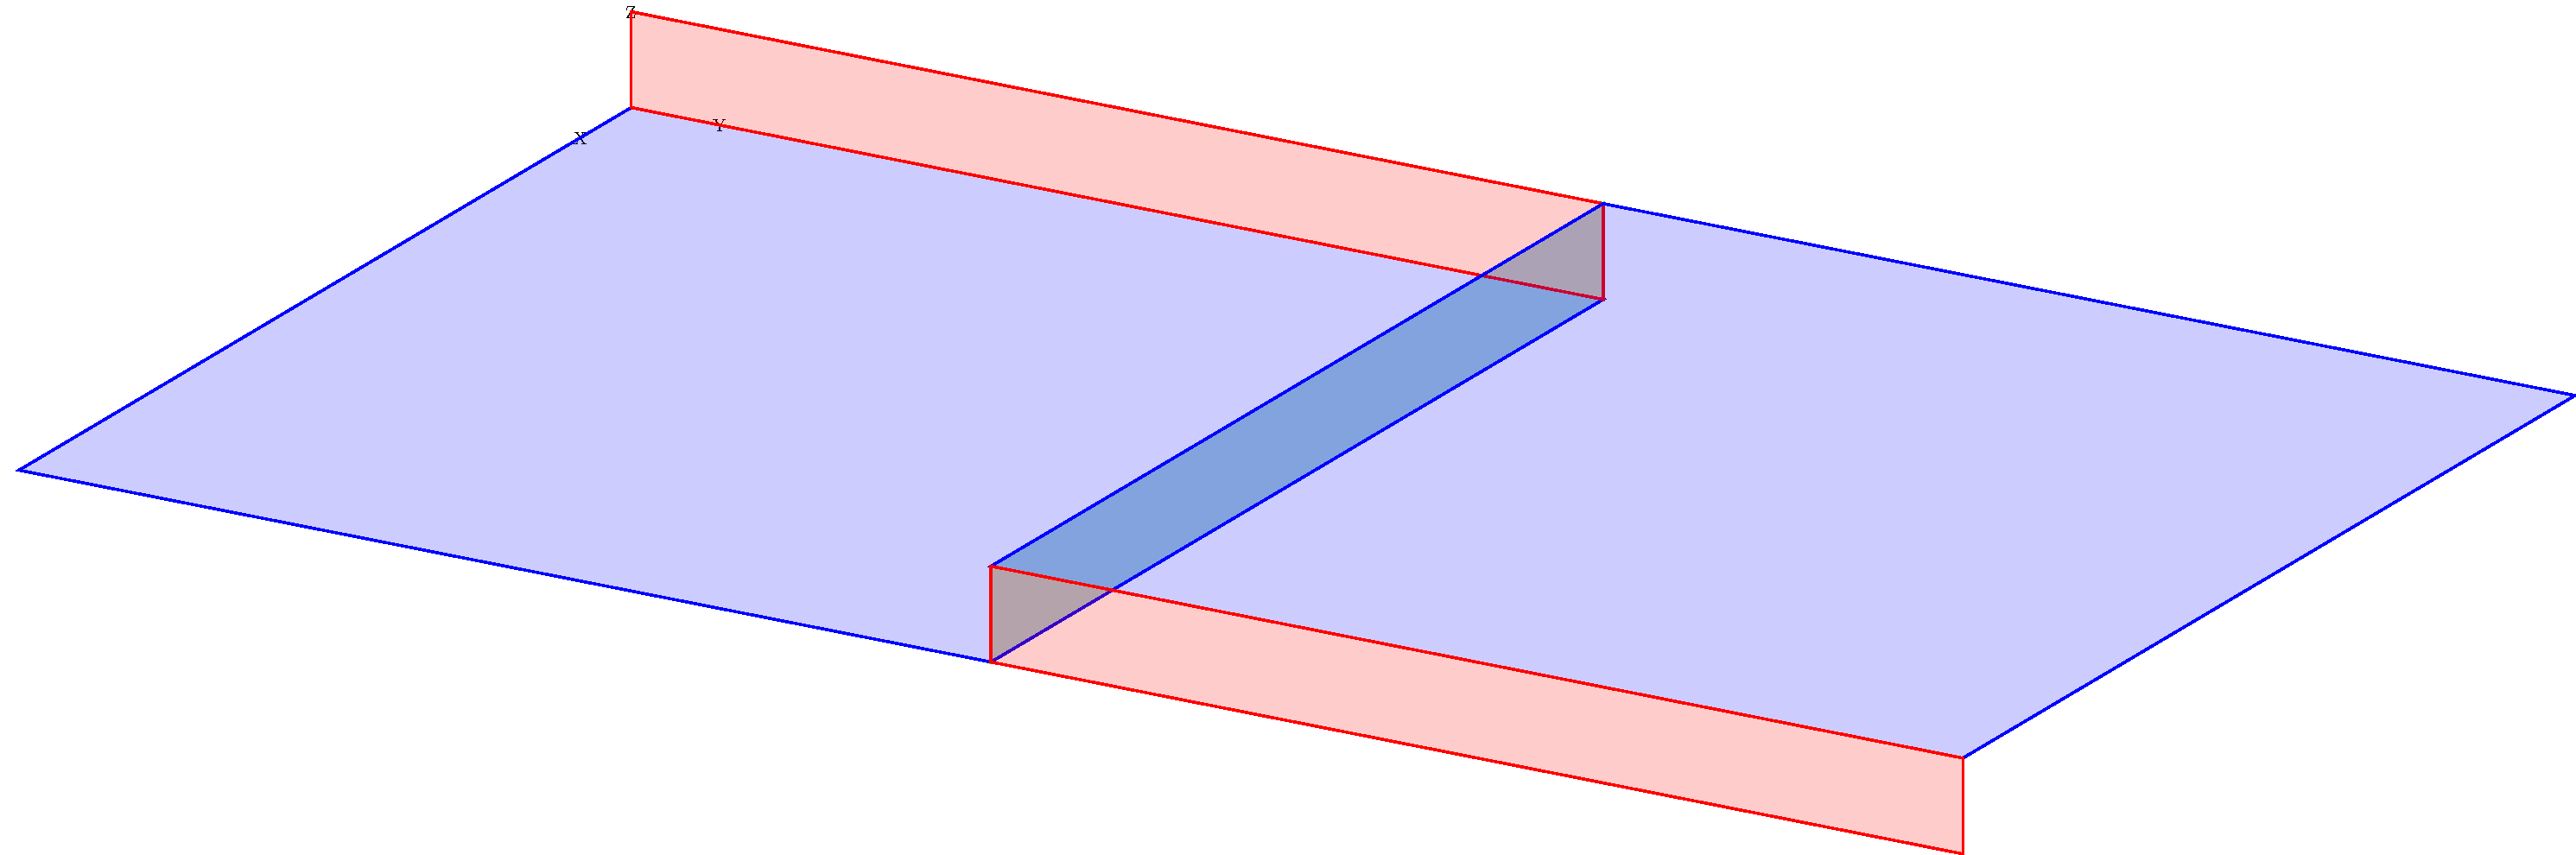
\includegraphics[width=\textwidth]{figures/7/12x21x2_manifold_3d.pdf}
	\caption{A manifold of $G= (12,21,2)$.}
	\label{}
\end{subfigure} \hfill%
\begin{subfigure}{0.45\textwidth}
	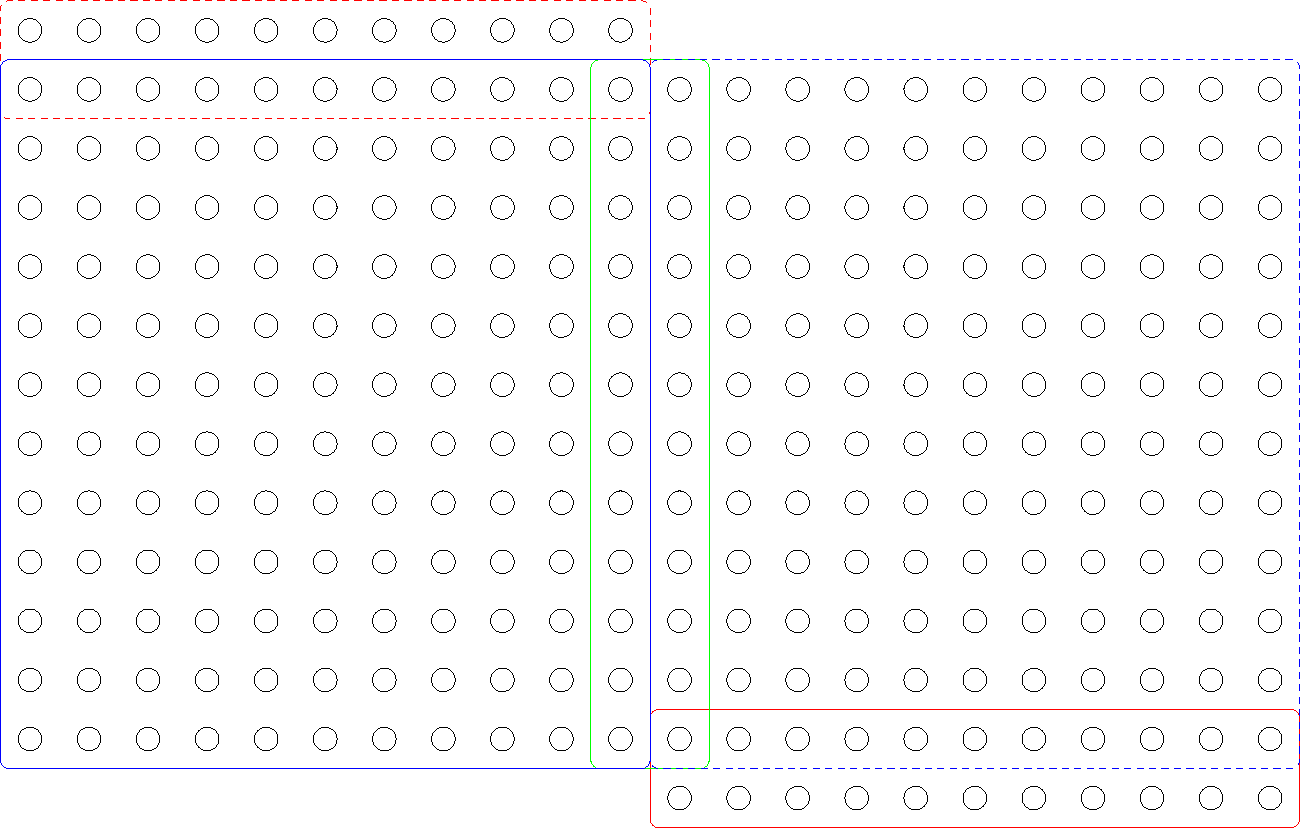
\includegraphics[width=\textwidth]{figures/7/12x21x2_unfolded.pdf}
	\caption{A proper unfolding of $G$.}
	\label{}
\end{subfigure}
\caption{A proper unfolding of $G= (12,21,2)$. Colored rectangles indicate faces of $G$. Dashed lines indicate that cells appear on different layers. }
\label{fig:12x21x2_unfolded}
\end{figure} 

\begin{figure}[]
\centering
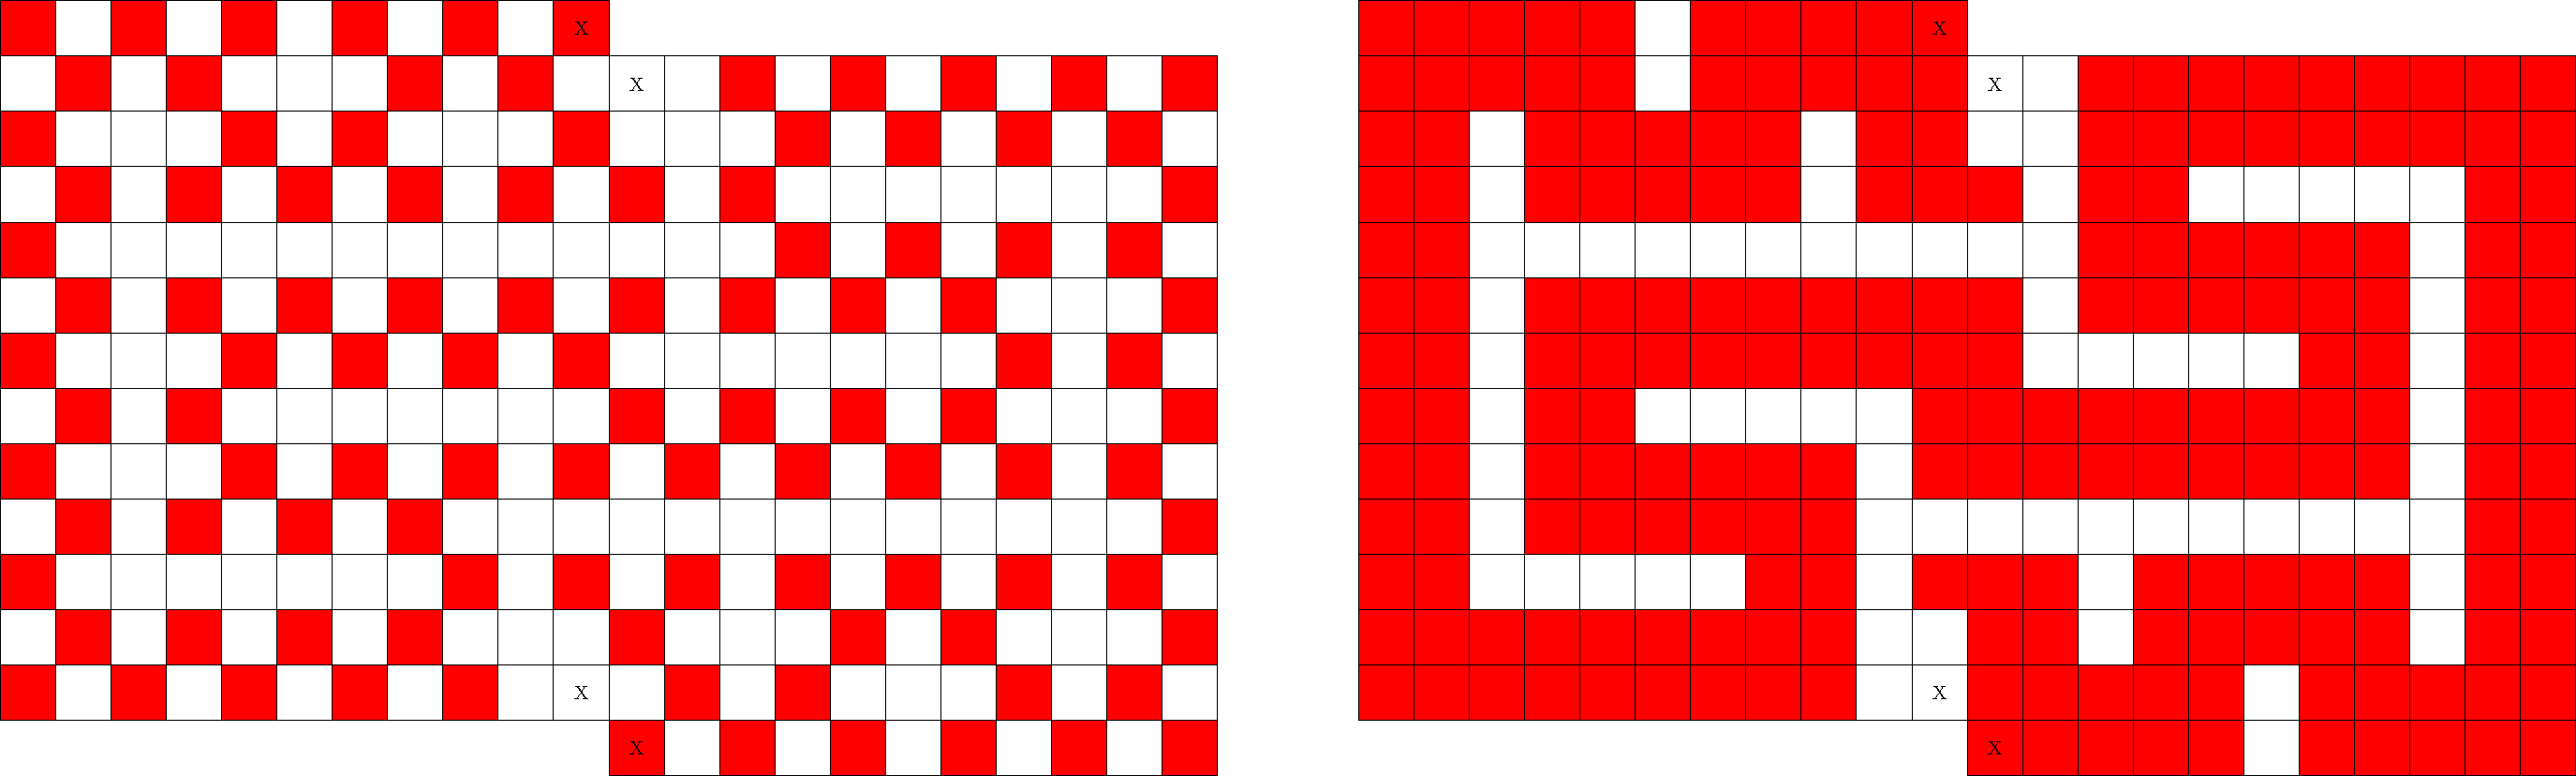
\includegraphics[width=0.8\textwidth]{figures/7/12x21x2_unfolded_lethal.pdf}
\caption{A percolating set on the proper unfolding of $G= (12,21,2)$.}
\label{fig:12x21x2_unfolded_lethal}
\end{figure} 

\end{comment}
% COMMENT
% COMMENT
% COMMENT

\section{Thickness 3}

\begin{con}
\label{con:3x3xeven}
All tuples $(a,3,3)$ with $a \equiv 0 \pmod 2$ and $a > 2$ are perfect. 
\end{con}

\begin{proof}
Let $G=G(2k,3,3)$ be a grid such that $k > 1$. Let $A = \{1,2,3\} \times [3] \times [3]$, $B = \{2k\} \times [3] \times [3]$, and $X_i = \{2i+2,2i+3\} \times [3] \times [3]$ for $i \in [k-2]$, be regions of $G$. Denote by $AX^kB$ the union of regions $A \cup X_1 \cup \dots \cup X_{k} \cup B$, and note that $G=AX^kB$. Let $A_t^k \subseteq V(G)$ be the set of infected vertices in $G$ at time $t$, and suppose that each $X_i$ contains the same pattern of infected vertices (see Figure \ref{fig:3x6x3}). We show that $A_0^k$ is lethal and perfect. 

Consider the union of regions $AX^k = A \cup X_1 \cup \dots \cup X_{k}$ (see Figure \ref{fig:3x13x3}). Let $L_1$, $L_2$ and $L_3$ be the top, middle and bottom levels of $AX^k$, respectively. Observe that after one time-step, the subgraph of $L_2 \setminus \{2k-1\} \times [3] \times \{2\}$ induced by $\overline{A_1^k}$ is acyclic with no border-to-border vertices, and so by Proposition \ref{prop:immune_regions}, $A_0^k$ infects all vertices of $L_2$ apart from those in the rightmost column (labeled ``X"; see Figure \ref{fig:3x13x3}). Therefore, by Lemma \ref{lem:2_neighbor_levels}, all vertices in $L_1$ apart from the rightmost column (labeled ``Y") become infected by the 2-neighbor process. Similarly, the red arrow in Figure \ref{fig:3x13x3}) shows the path of infection in $L_3$. 

Consider these observations in the context of $G$. Figure \ref{fig:3x14x3} shows that it takes 7 additional time steps to fully infect $L_1$ and $L_2$. By Lemma \ref{lem:2_neighbor_levels}, the remaining healthy vertices in $L_3$ become infected. We therefore conclude that $A_0^k$ is lethal on $G$ under the 3-neighbor process.

To prove that $A_0^k$ is perfect, observe that $|A_0^k| = 8 + 4(k-2) + 3=4k+3$. The surface area bound for $G(2k,3,3)$ is given by
$$\frac{(2k)(3) + (3)(3) + (3)(2k)}{3} = \frac{12k + 9}{3} = 4k+3.$$
Since these two values are equal, $A_0^k$ is tight and lethal, and therefore perfect.
\end{proof}

\begin{figure}[]
\centering
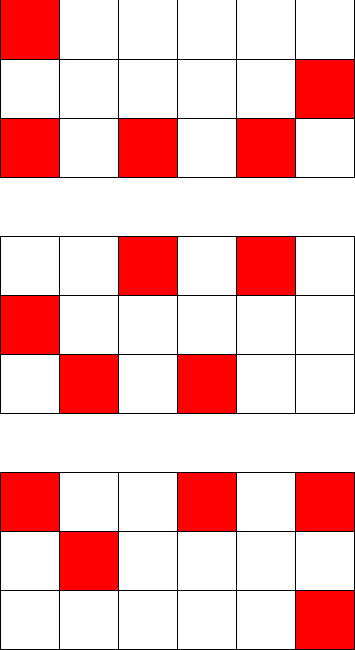
\includegraphics[width=0.2\textwidth]{figures/7/3x6x3.pdf}
\caption{The regions $A$, $X$, $B$ on $G=AXB$ with infected set $A_0$.}
\label{fig:3x6x3}
\end{figure} 

\begin{figure}[]
\centering
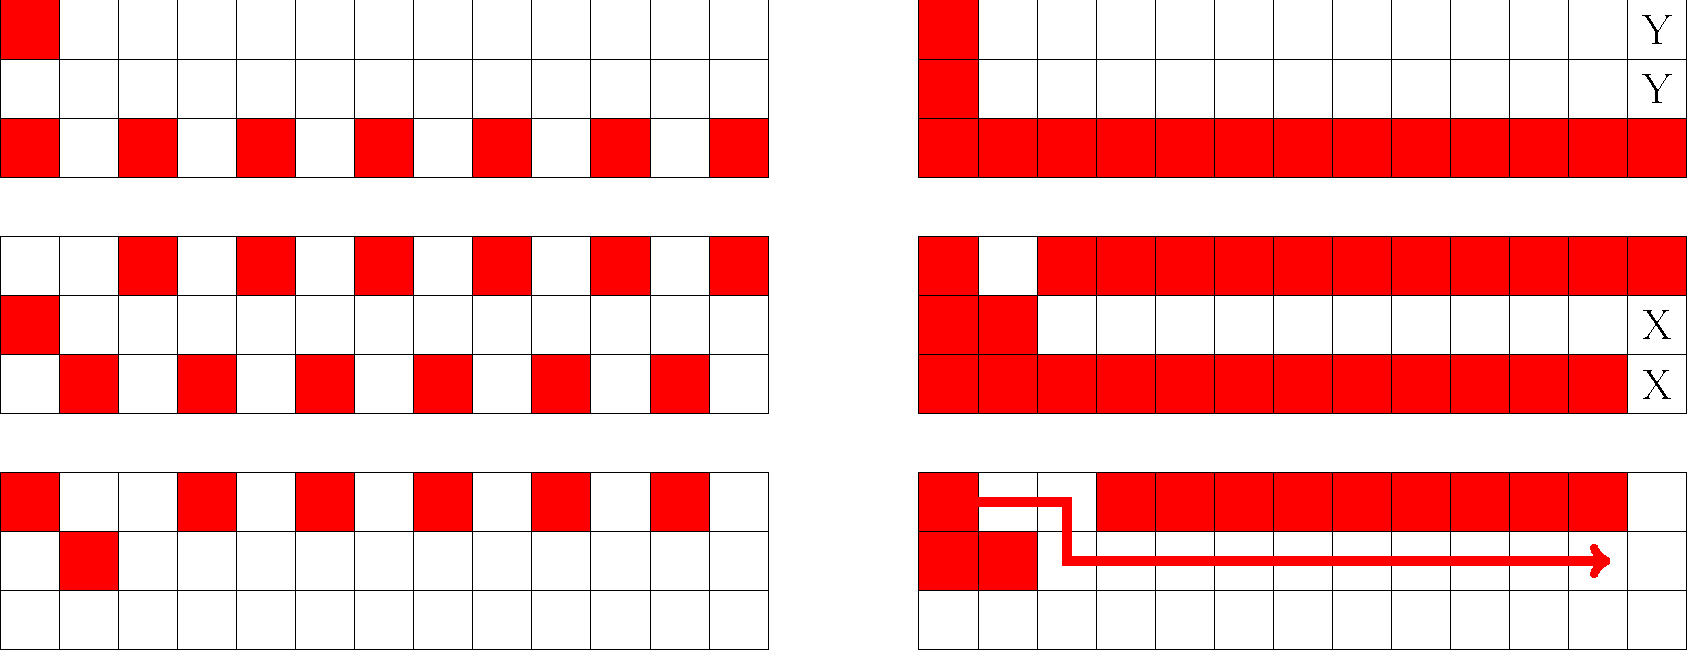
\includegraphics[width=0.8\textwidth]{figures/7/3x13x3.pdf}
\caption{An infection on $AX^5$, $t=0$ and $t=1$.}
\label{fig:3x13x3}
\end{figure} 

\begin{figure}[]
\centering
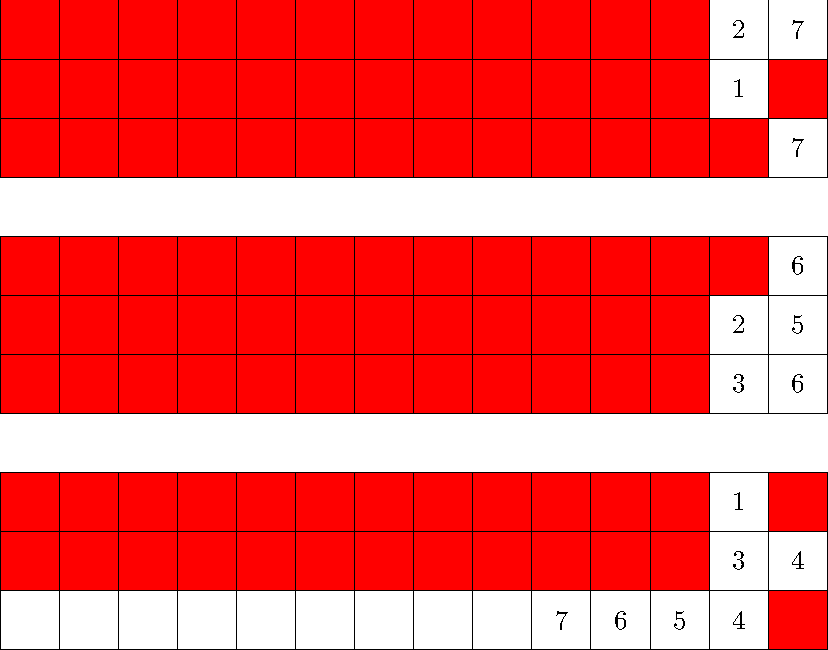
\includegraphics[width=0.5\textwidth]{figures/7/3x14x3_numbered_heatmap.pdf}
\caption{Time steps of a perfect lethal infection on $G(3,14,3)$.}
\label{fig:3x14x3}
\end{figure} 

\begin{con}
\label{con:3xaxb}
All tuples $(a,b,3)$ with $a \equiv 3 \pmod 6$, $b \equiv 1 \pmod 2$ and $a,b \geq 3$ are perfect. 
\end{con}

\begin{proof}
Consider the grid $H=G(a+2,b+2,1)$, where $a \equiv 3 \pmod 6$ and $b \equiv 1 \pmod 2$. Observe that $H$ admits an optimal percolating set by Construction \ref{con:snake}, and that
$$\text{SA}(a,b,3) = \ceil{\text{SA}(a+2,b+2,1)} - 3.$$
We show that a proper unfolding of $G$ can be obtained from a simple augmentation of $H$. Let $H'$ be the grid obtained by deleting the four vertices in the bottom, right-most corner of $H$ (see Figure \ref{fig:17x25x1_unfolded}). Consider the folding pattern illustrated in Figure \ref{fig:17x25x1_manifold}, and observe that the pairs of vertices adjacent to the deleted region are duplicates of each other. (In other words, consider folding up the red and green regions in Figure \ref{fig:17x25x1_manifold}, and notice that this operation causes vertices to overlap.) Taking this into account, $H'$ percolates by Proposition \ref{prop:immune_regions}. Since $H$ admits an optimal percolating set of size $\ceil{\text{SA}(a+2,b+2,1)}$, and precisely 3 of the vertices deleted from $H$ to obtain $H'$ were infected, it follows that $H'$ admits a perfect lethal set. Finally, by Lemma \ref{cor:three_walls}, $G$ is perfect.
\end{proof}

\begin{figure}[]
\centering
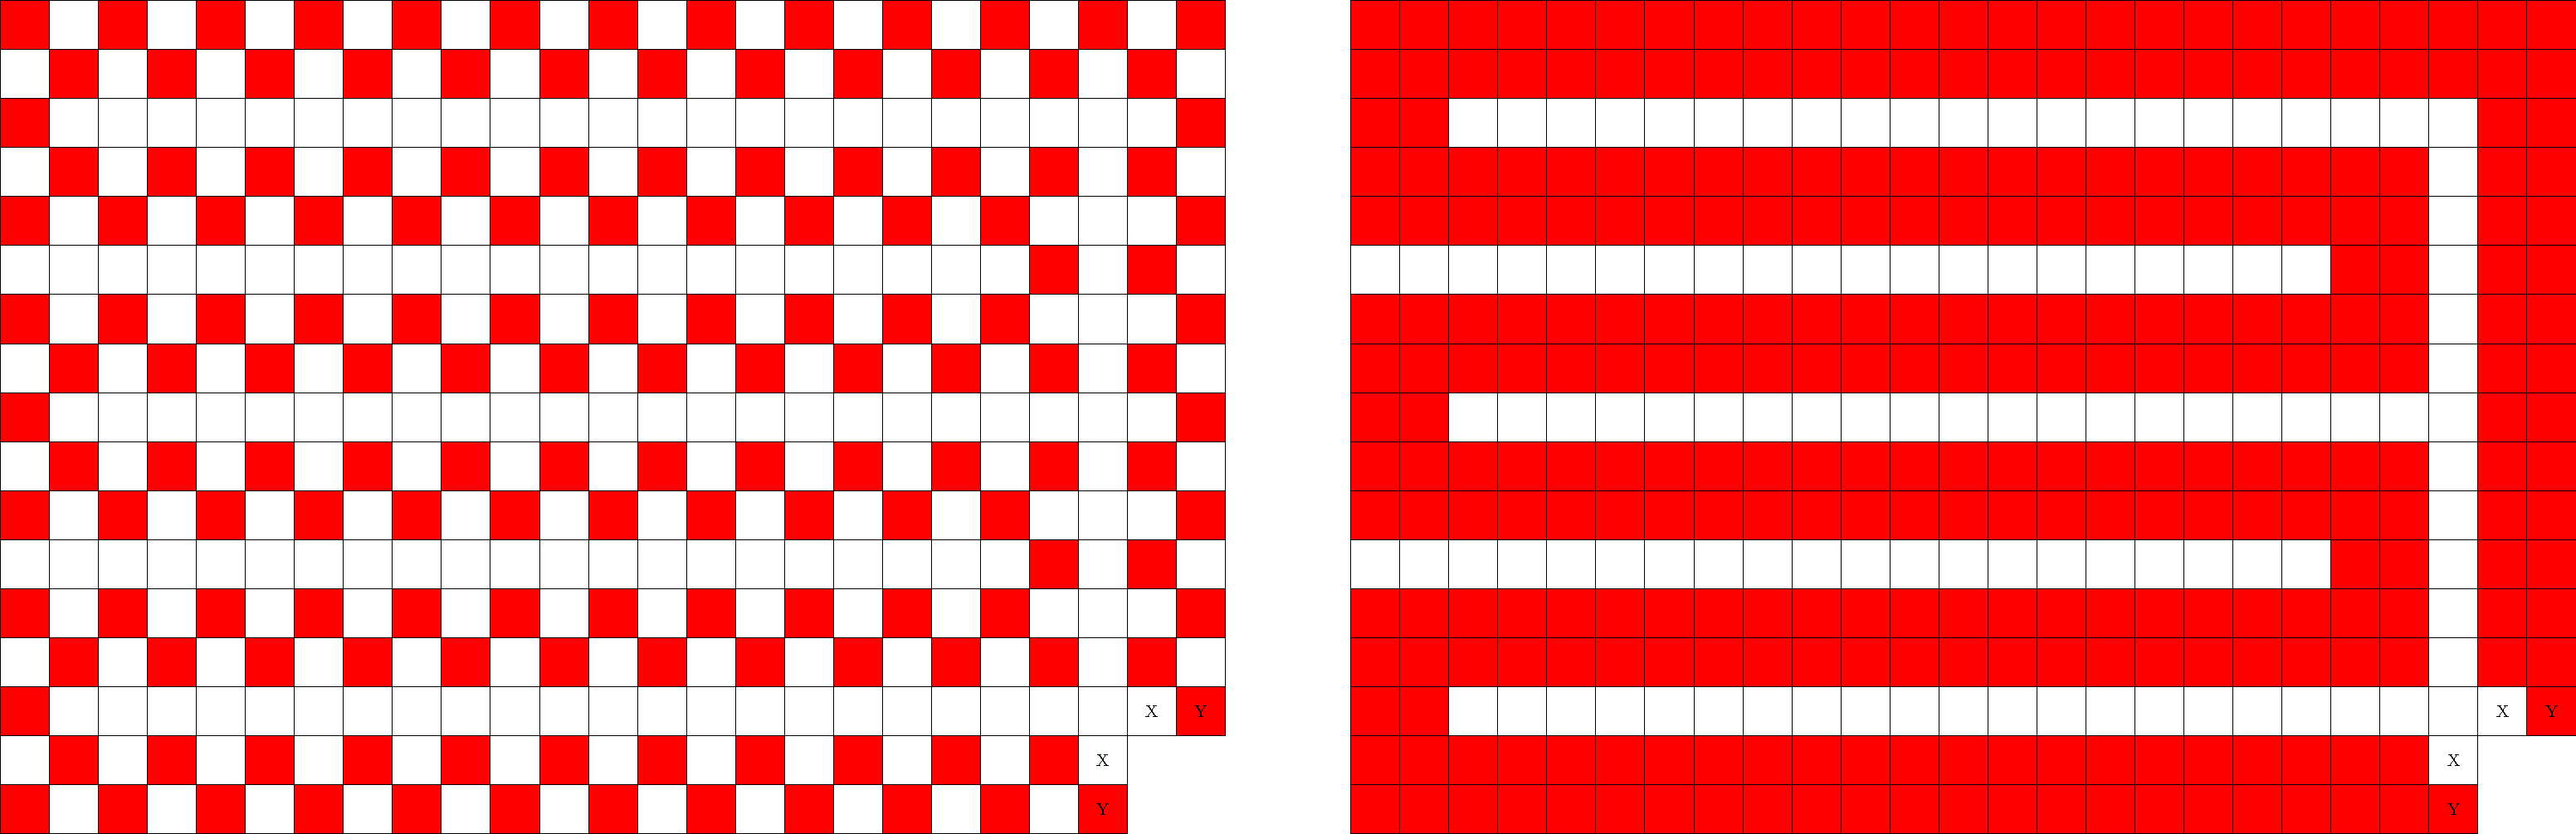
\includegraphics[width=0.8\textwidth]{figures/7/17x25x1_unfolded.pdf}
\caption{A percolating set on the proper unfolding $H'$ of $G(15,23,3)$.}
\label{fig:17x25x1_unfolded}
\end{figure}

\begin{figure}[]
\centering
\begin{subfigure}{0.45\textwidth}
	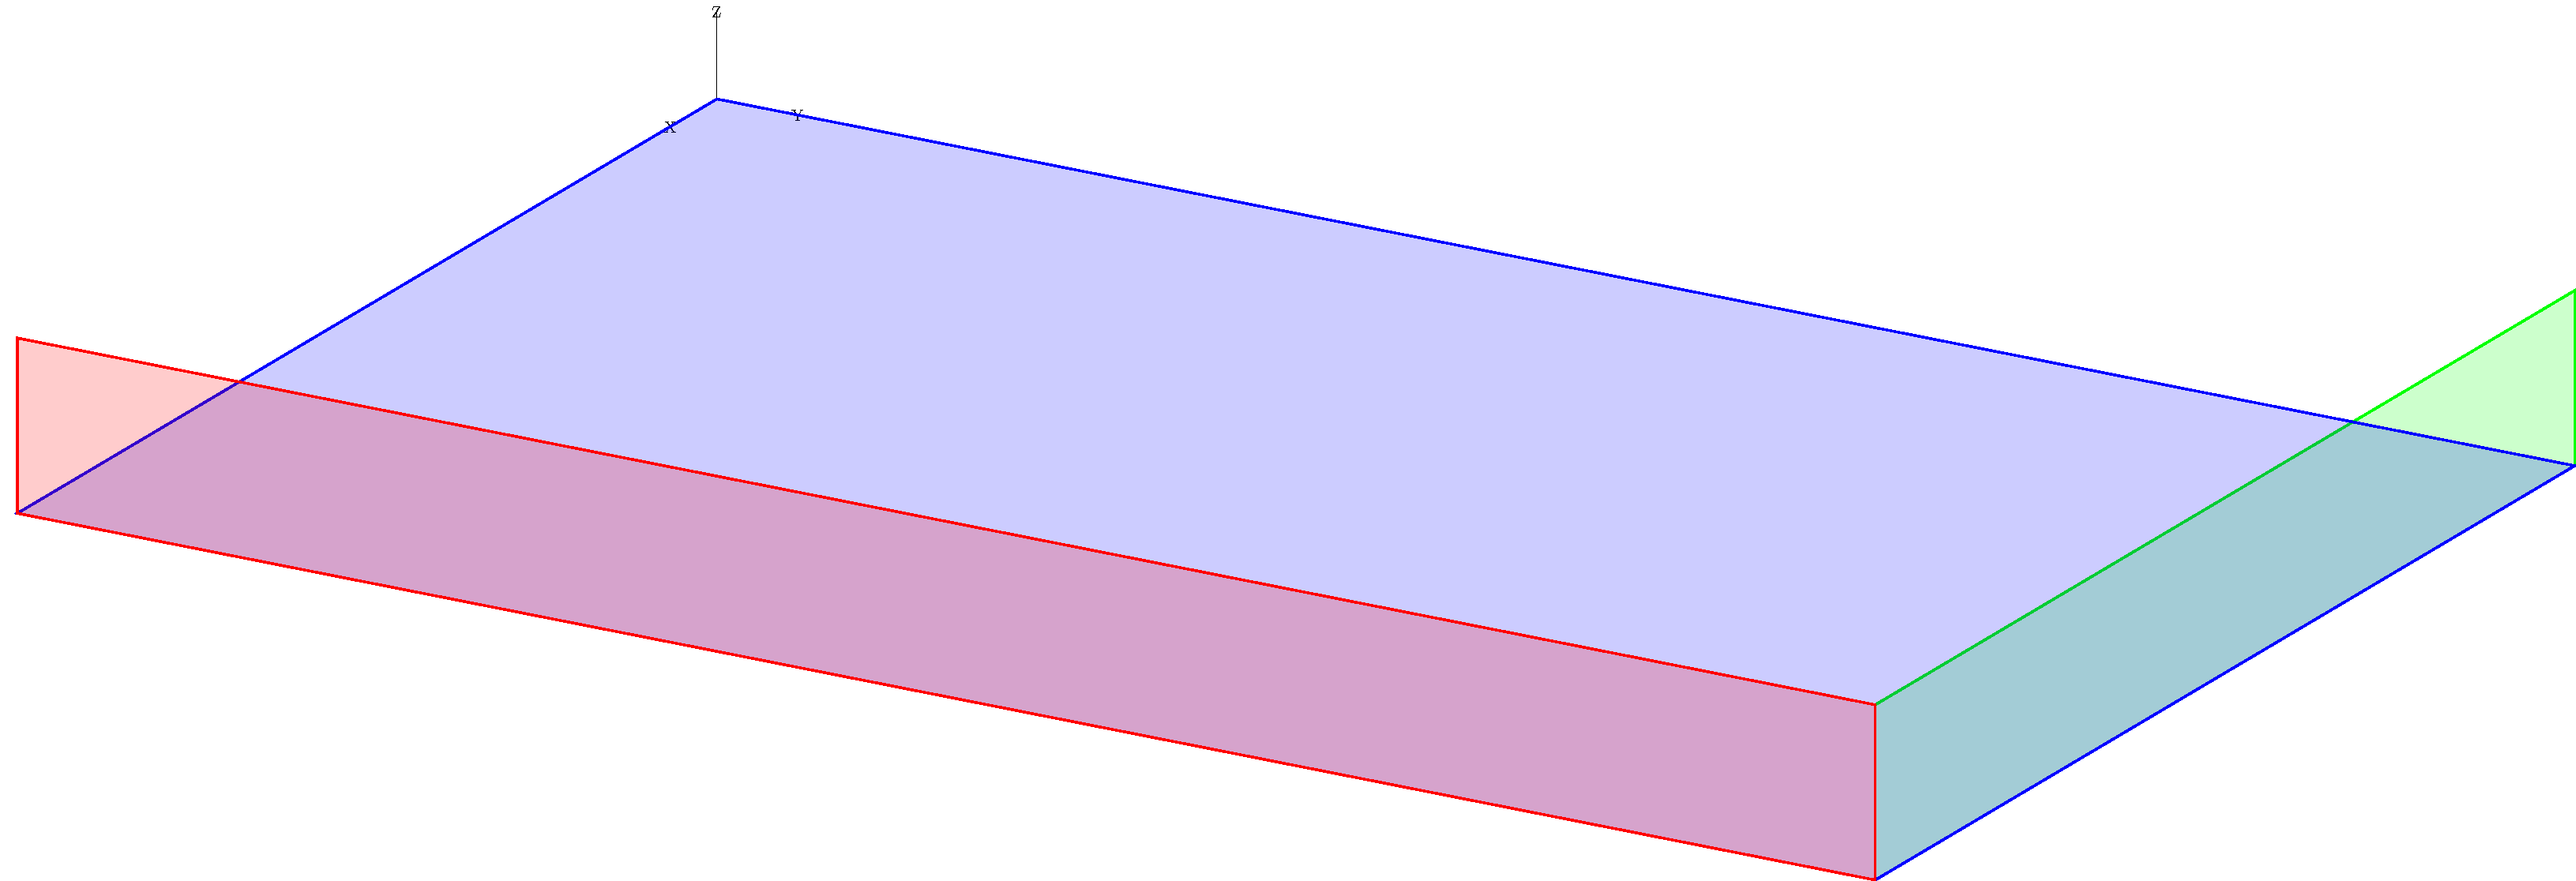
\includegraphics[width=\textwidth]{figures/7/17x25x1_manifold_3d.pdf}
	\caption{A manifold of $G(15,23,3)$.}
	\label{}
\end{subfigure} \hfill%
\begin{subfigure}{0.45\textwidth}
	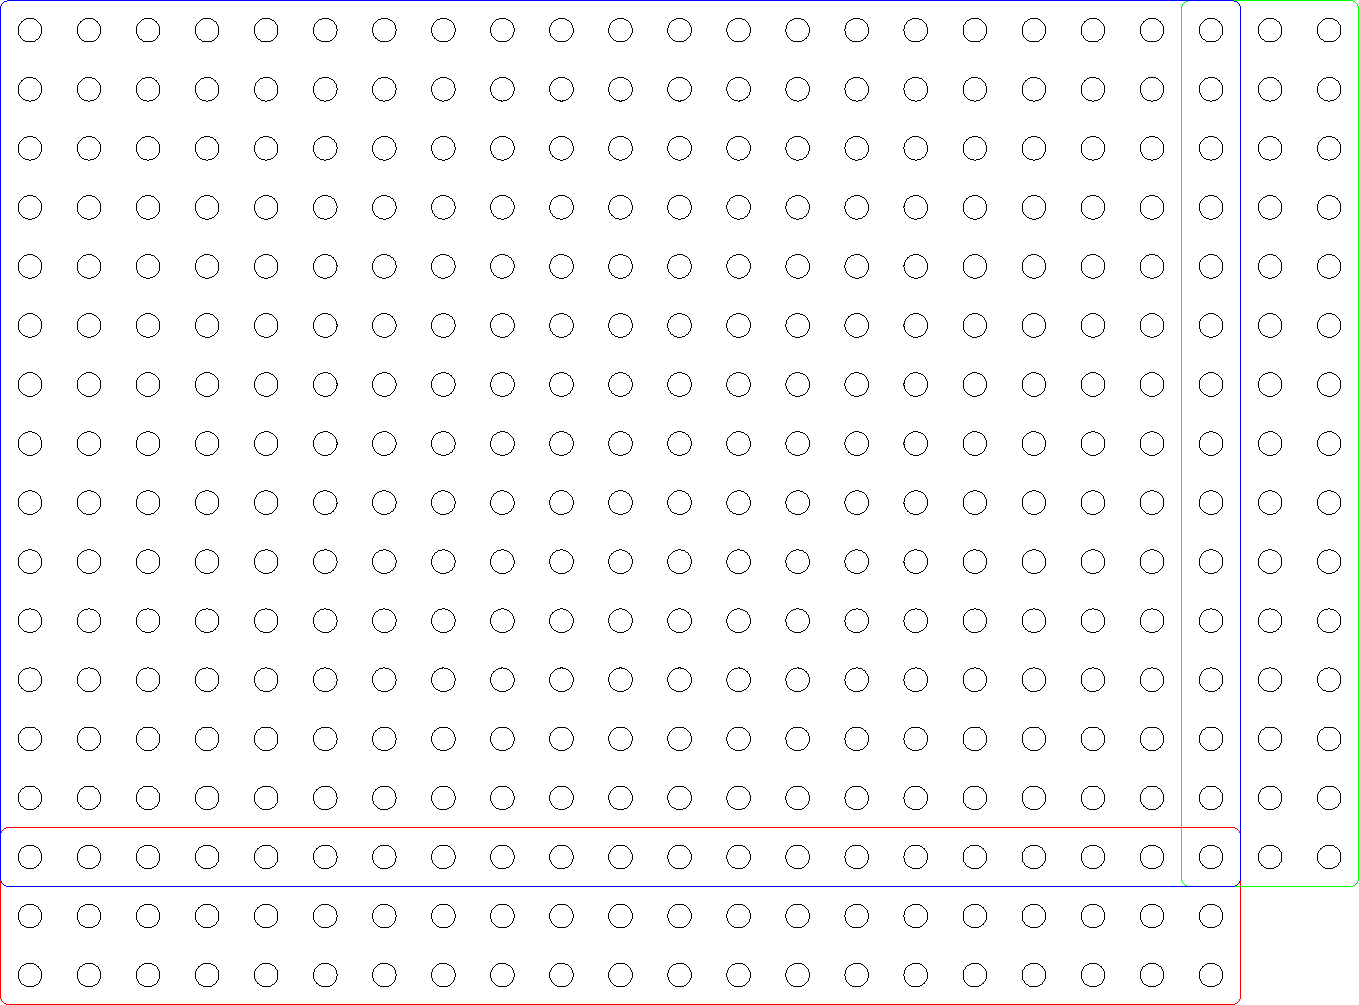
\includegraphics[width=\textwidth]{figures/7/17x25x1_manifold.pdf}
	\caption{A proper unfolding of $G$.}
	\label{}
\end{subfigure}
\caption{A proper unfolding of $G(15,23,3)$. Colored rectangles indicate faces of $G$. }
\label{fig:17x25x1_manifold}
\end{figure} 

\begin{con}
\label{con:3x4xa}
All tuples $(a,4,3)$ with $a \equiv 3 \pmod 6$ and $a \geq 9$ are perfect. 
\end{con}

\begin{proof}
Let $G=G(6k+3,4,3)$ be a grid such that $k \geq 1$, and let $X_1, \dots, X_{k}$ be the repeated regions of $G$ in the $x$-direction. Denote the union of these components by $X^k$. Let $A_t^k \subseteq V(G)$ be the set of infected vertices in $G$ at time $t$, and suppose that each $X_i$ contains the same pattern of infected vertices (see Figure \ref{fig:4x15x3}). We show that $A_0^k$ is lethal and perfect. 

Let $L_1$, $L_2$ and $L_3$ be the top, middle and bottom levels of $G$, respectively. Consider $L_3$ at $t=1$ (see Figure \ref{fig:4x15x3}). Observe that the vertices labeled ``X" are infected at $t=2$, and subsequently all vertices in $X^k \cap L_3$ (with the exception of the vertex labeled ``Y") are infected by Proposition \ref{prop:immune_regions}. Additionally, the infected vertices in $L_2$ at $t=1$ are lethal in $X^k \cap L_2$ under the 2-neighbor process, and so by Lemma \ref{lem:2_neighbor_levels}, all vertices of $X^k \cap L_2$ (apart from the one labeled ``Y") are infected.

Consider these observations in the context of $G$. Figure \ref{fig:4x15x3_timesteps} shows that it takes 5 additional time steps to fully infect $L_2$. By Lemma \ref{lem:2_neighbor_levels}, the remaining healthy vertices in $L_1$ and $L_3$ become infected. We therefore conclude that $A_0^k$ is lethal on $G$ under the 3-neighbor process.

To prove that $A_0^k$ is perfect, observe that for $i \in [k]$, each $X_i$ contains 14 infected vertices. Of the remaining vertices in $G$, 11 are infected. Therefore, $|A_0| = 14k+11$. The surface area bound for $G(6k+3,4,3)$ is given by
$$\frac{(6k+3)(4) + (4)(3) + (3)(6k+3)}{3} = \frac{42k + 33}{3} = 14k+11.$$
Since these two values are equal, $A_0^k$ is tight and lethal, and therefore perfect.
\end{proof}

\begin{figure}[]
\centering
\begin{subfigure}{0.65\textwidth}
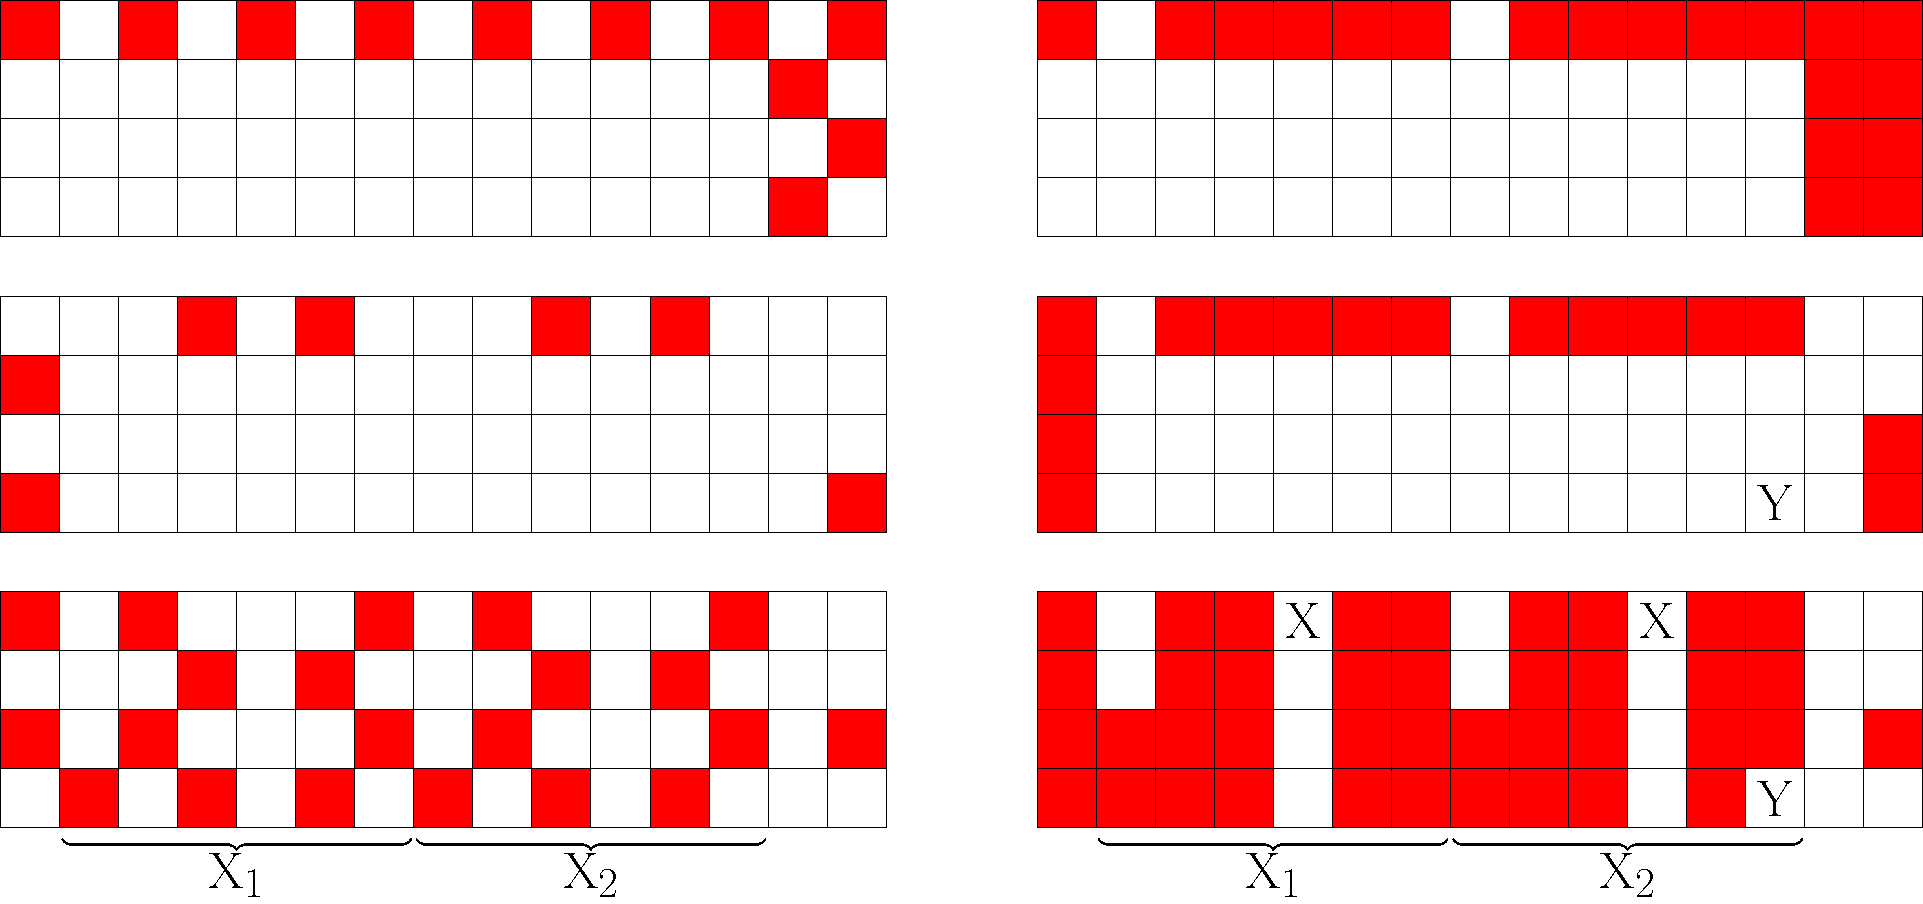
\includegraphics[width=\textwidth]{figures/7/4x15x3.pdf}
\caption{A lethal set on $(4,15,3)$, $t=0$ and $t=1$.}
\label{fig:4x15x3}
\end{subfigure} \hfill%
\begin{subfigure}{0.3\textwidth}
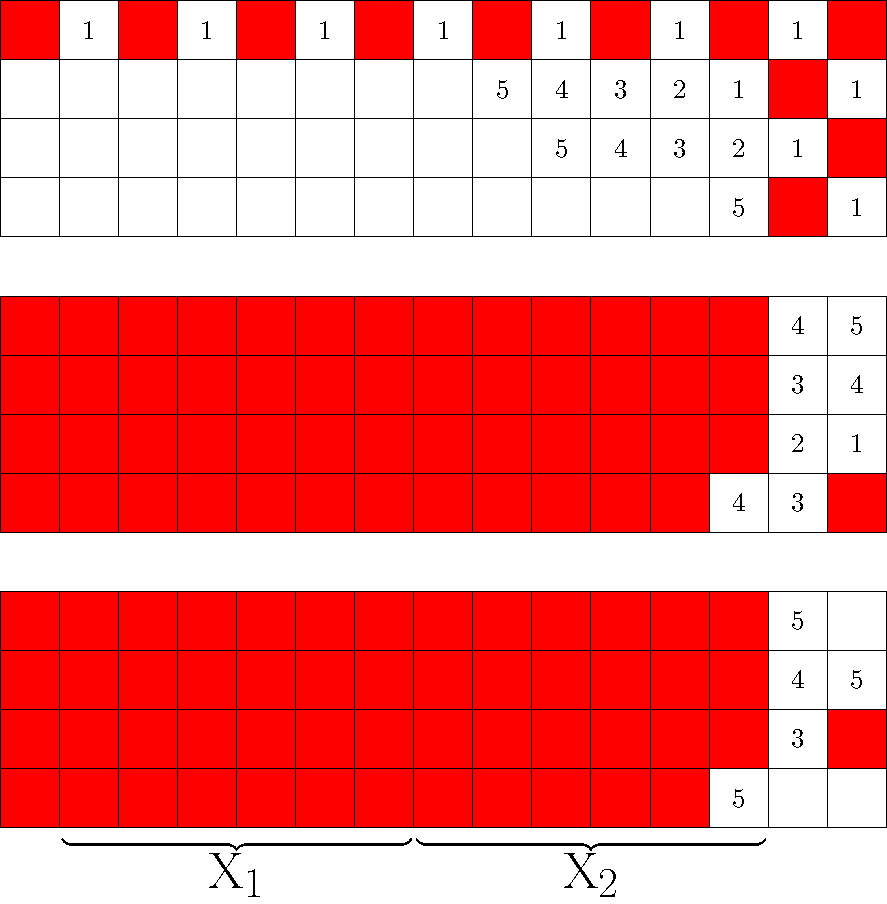
\includegraphics[width=\textwidth]{figures/7/4x15x3_timesteps_numbered_heatmap.pdf}
\caption{Time steps to infect $L_2$.}
\label{fig:4x15x3_timesteps}
\end{subfigure}
\caption{Time steps of infection on $G(4,15,3)$.}
\label{fig:}
\end{figure} 

\begin{con}
\label{con:3x6xeven}
All tuples $(a,6,3)$ with $a \equiv 0 \pmod 2$ and $a \geq 4$ are perfect. 
\end{con}

\begin{proof}
Let $G=G(2k+2,6,3)$ be a grid such that $k \geq 1$, and let $X_1, \dots, X_{k}$ be the repeated regions of $G$ in the $x$-direction. Denote the union of these regions by $X^k$. Let $A_t^k \subseteq V(G)$ be the set of infected vertices in $G$ at time $t$, and suppose that each $X_i$ contains the same pattern of infected vertices (see Figure \ref{fig:6x12x3}). We show that $A_0^k$ is lethal and perfect. 

Let $L_1$, $L_2$ and $L_3$ be the top, middle and bottom levels of $G$, respectively. Consider $L_2$ at $t=1$ (see Figure \ref{fig:6x12x3}). Observe that all vertices in $X^k \cap L_2$ are infected by Lemma \ref{lem:2_neighbor_levels}, due to adjacent infected vertices in $L_1$ and $L_3$. 

Consider these observations in the context of $G$. Figure \ref{fig:6x12x3_timesteps} shows that it takes 2 additional time steps to fully infect $L_2$. Since $L_1$ and $L_3$ contain lethal sets under the 2-neighbor process, by Lemma \ref{lem:2_neighbor_levels}, the remaining healthy vertices in these levels become infected. We therefore conclude that $A_0^k$ is lethal on $G$ under the 3-neighbor process.

To prove that $A_0^k$ is perfect, observe that for $i \in [k]$, each $X_i$ contains 6 infected vertices. Of the remaining vertices in $G$, 12 are infected. Therefore, $|A_0| = 6k+12$. The surface area bound for $G(2k+2,6,3)$ is given by
$$\frac{(2k+2)(6) + (6)(3) + (3)(2k+2)}{3} = \frac{18k + 36}{3} = 6k+12.$$
Since these two values are equal, $A_0^k$ is tight and lethal, and therefore perfect.
\end{proof}

\begin{figure}[]
\centering
\begin{subfigure}{0.65\textwidth}
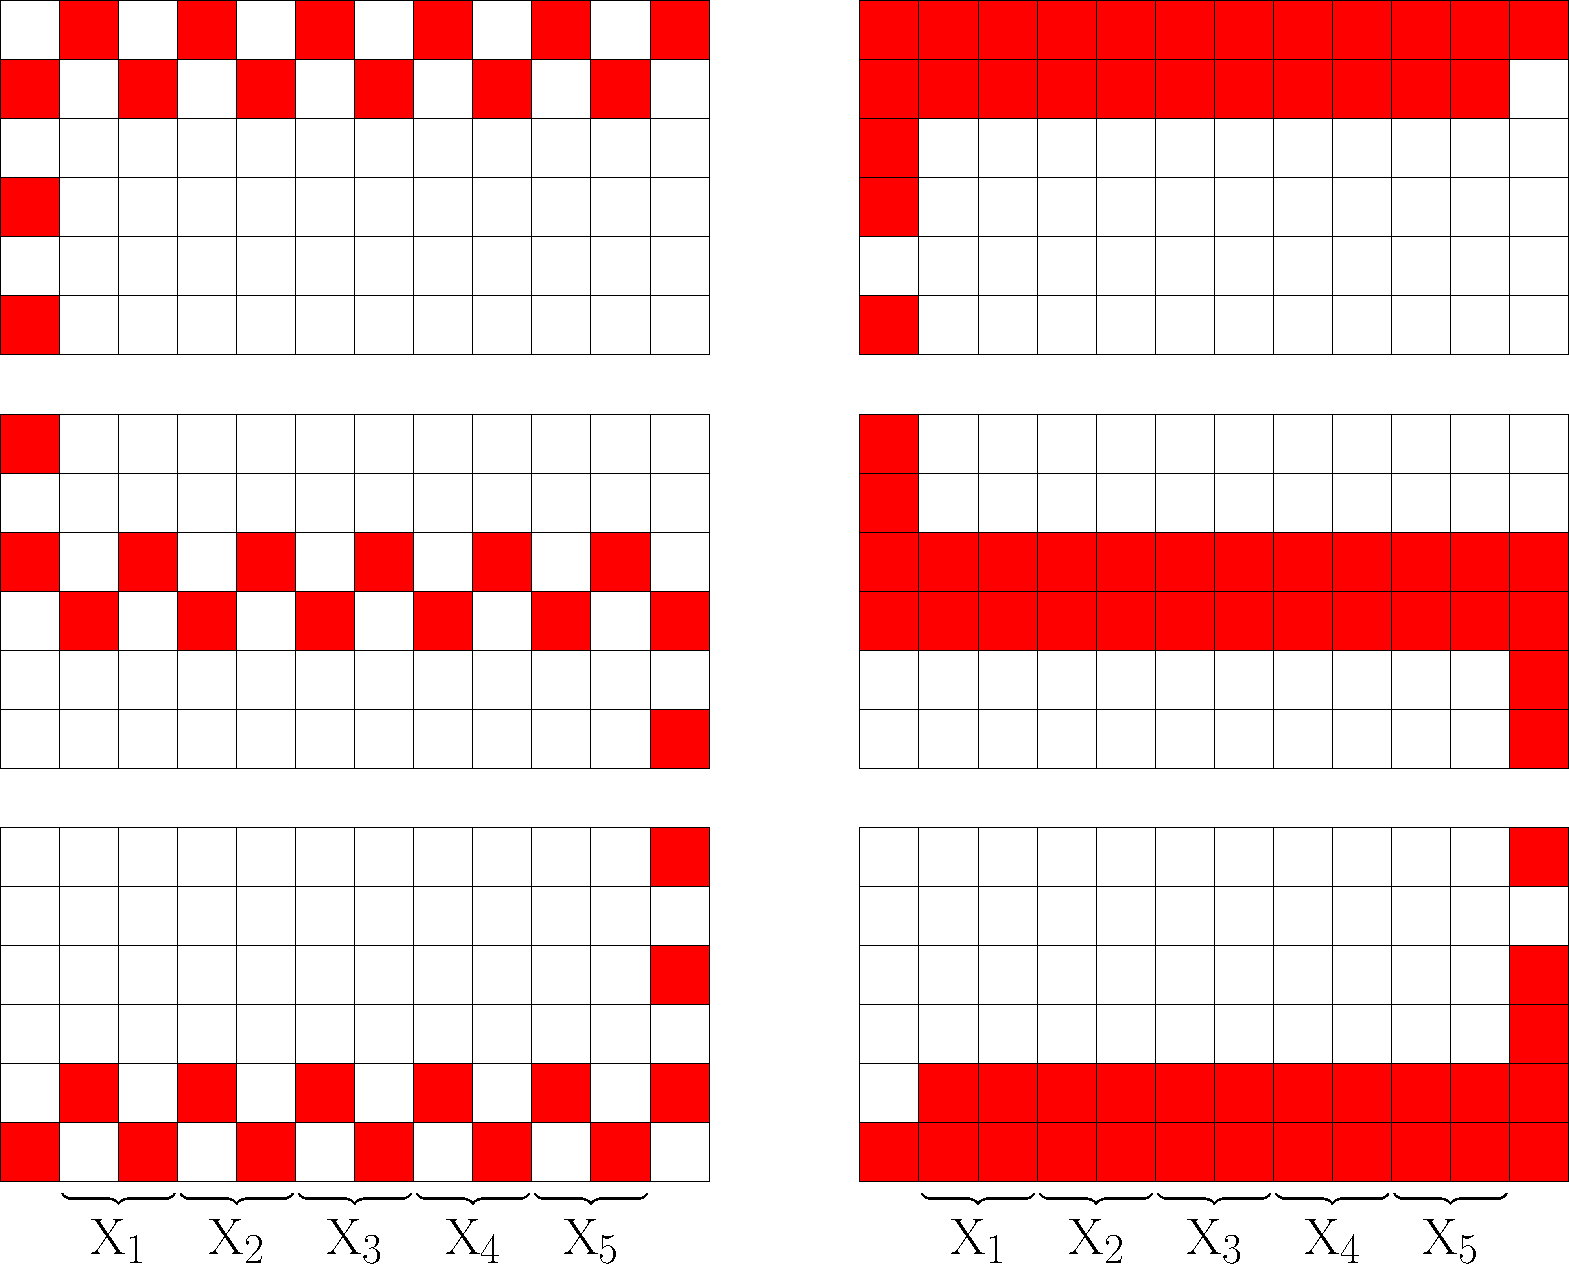
\includegraphics[width=\textwidth]{figures/7/6x12x3.pdf}
\caption{A lethal set on $(6,12,3)$, $t=0$ and $t=1$.}
\label{fig:6x12x3}	
\end{subfigure} \hfill%
\begin{subfigure}{0.2915\textwidth}
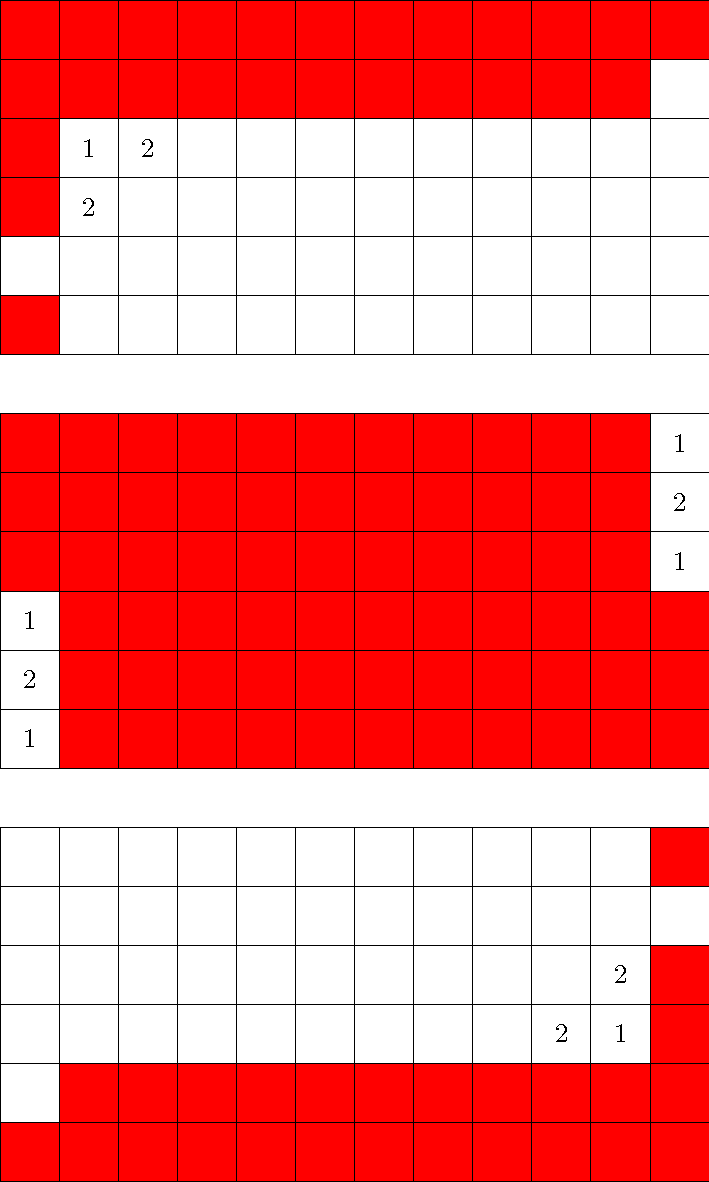
\includegraphics[width=\textwidth]{figures/7/6x12x3_L2_numbered_heatmap.pdf}
\caption{Time steps to infect $L_2$.}
\label{fig:6x12x3_timesteps}
\end{subfigure}
\caption{Time steps of infection on $G(6,12,3)$.}
\label{fig:}
\end{figure} 

\begin{con}
\label{con:3x6xodd}
All tuples $(a,6,3)$ with $a \equiv 1 \pmod 2$ and $a \geq 5$ are perfect. 
\end{con}

\begin{proof}
Let $G=G(2k+3,6,3)$ be a grid such that $k \geq 1$, and let $X_1, \dots, X_{k}$ be the repeated regions of $G$ in the $x$-direction. Denote the union of these components by $X^k$. Let $A_t^k \subseteq V(G)$ be the set of infected vertices in $G$ at time $t$, and suppose that each $X_i$ contains the same pattern of infected vertices (see Figure \ref{fig:6x11x3}). We show that $A_0^k$ is lethal and perfect. 

Let $L_1$, $L_2$ and $L_3$ be the top, middle and bottom levels of $G$, respectively. Consider $L_2$ at $t=1$ (see Figure \ref{fig:6x11x3}). Observe that all vertices in $X^k \cap L_2$ (with the exception of the one labeled ``X") are infected by Lemma \ref{lem:2_neighbor_levels}, due to adjacent infected vertices in $L_1$ and $L_3$. 

Consider these observations in the context of $G$. Figure \ref{fig:6x11x3_timesteps} shows that it takes 5 additional time steps to fully infect $L_2$. Since $L_1$ and $L_3$ contain lethal sets under the 2-neighbor process, by Lemma \ref{lem:2_neighbor_levels}, the remaining healthy vertices in these levels become infected. We therefore conclude that $A_0^k$ is lethal on $G$ under the 3-neighbor process.

To prove that $A_0^k$ is perfect, observe that for $i \in [k]$, each $X_i$ contains 6 infected vertices. Of the remaining vertices in $G$, 15 are infected. Therefore, $|A_0| = 6k+15$. The surface area bound for $G(2k+3,6,3)$ is given by
$$\frac{(2k+3)(6) + (6)(3) + (3)(2k+3)}{3} = \frac{18k + 45}{3} = 6k+15.$$
Since these two values are equal, $A_0^k$ is tight and lethal, and therefore perfect.
\end{proof}


\begin{figure}[]
\centering
\begin{subfigure}[t]{0.65\textwidth}
\centering
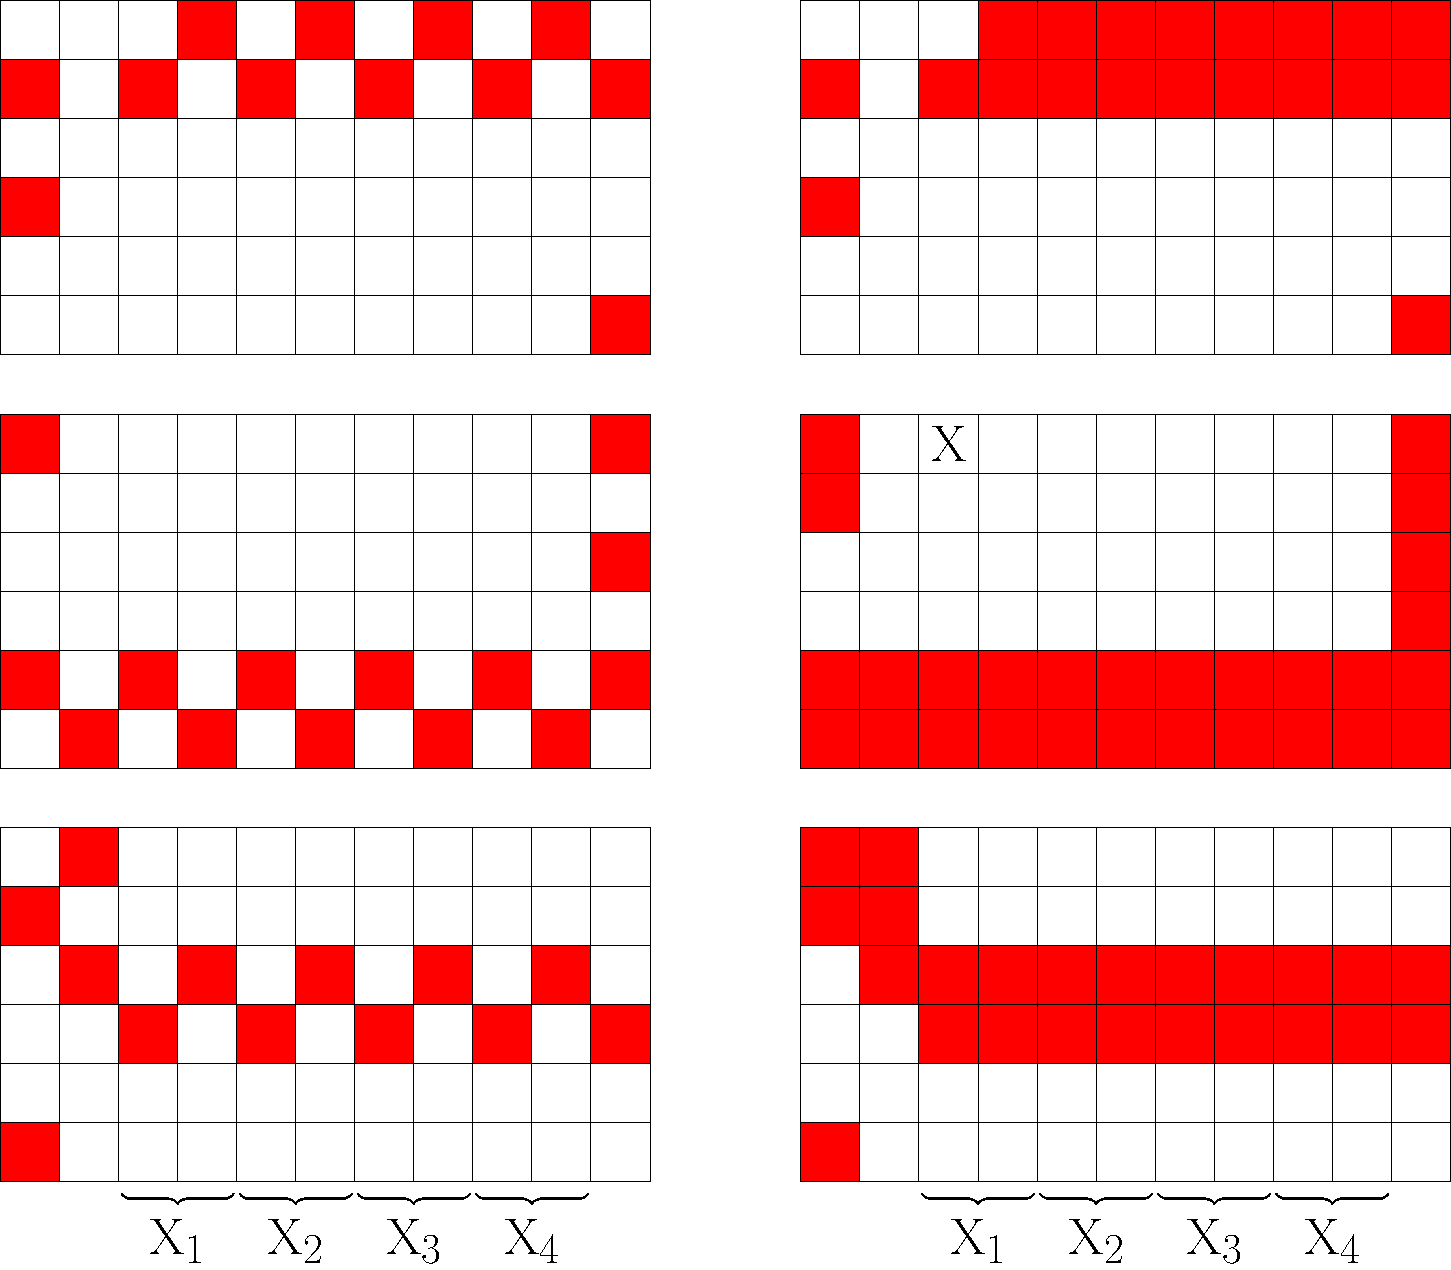
\includegraphics[width=\textwidth]{figures/7/6x11x3.pdf}
\caption{A lethal set on $G(6,11,3)$, $t=0$ and $t=1$.}
\label{fig:6x11x3}	
\end{subfigure} \hfill%
\begin{subfigure}[t]{0.2915\textwidth}
\centering
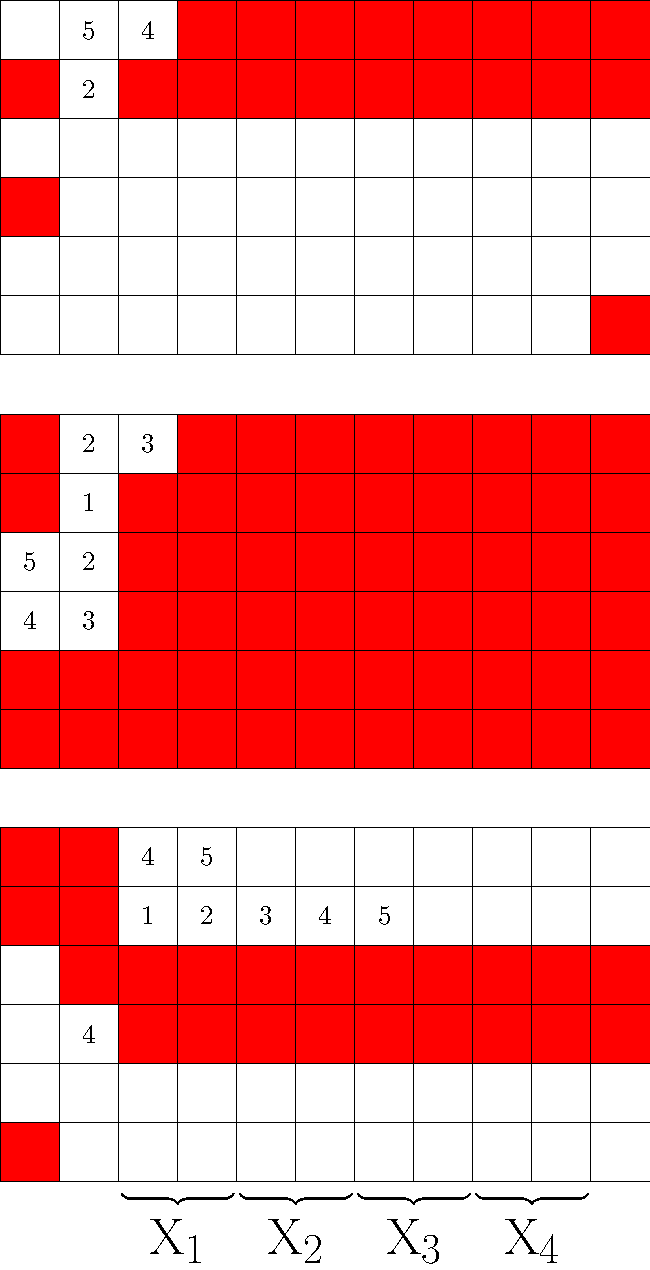
\includegraphics[width=\textwidth]{figures/7/6x11x3_L2_numbered_heatmap.pdf}
\caption{Time steps to infect $L_2$.}
\label{fig:6x11x3_timesteps}
\end{subfigure}
\caption{Time steps of infection on $G(6,11,3)$.}
\label{fig:}
\end{figure} 

% COMMENT
% COMMENT
% COMMENT
% COMMENT

\begin{comment}

\begin{figure}[]
\centering
\begin{subfigure}{0.45\textwidth}
	
\end{subfigure} \hfill%
\begin{subfigure}{0.45\textwidth}
	
\end{subfigure}
\caption{}
\label{fig:}
\end{figure} 

\section{Individual constructions}

In this section, we diagram lethal set constructions for single grids. The initial infection $A$ is colored red, and all other cells are labeled with the time $t$ that they are first infected. 

% (5, 2, 2)
\begin{con}
The grid $(5,2,2)$ is perfect.
\end{con}

\begin{proof}
See figure \ref{fig:2x5x2_numbered_heatmap}.
\end{proof}

\begin{figure}[]
\centering
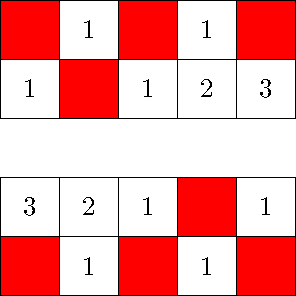
\includegraphics[width=0.2\textwidth]{figures/7/2x5x2_numbered_heatmap.pdf}
\caption{}
\label{fig:2x5x2_numbered_heatmap}
\end{figure} 

% (5, 5, 5)
\begin{con}
The grid $(5,5,5)$ is perfect.
\end{con}

\begin{proof}
See figure \ref{fig:5x5x5_numbered_heatmap}.
\end{proof}

\begin{figure}[]
\centering
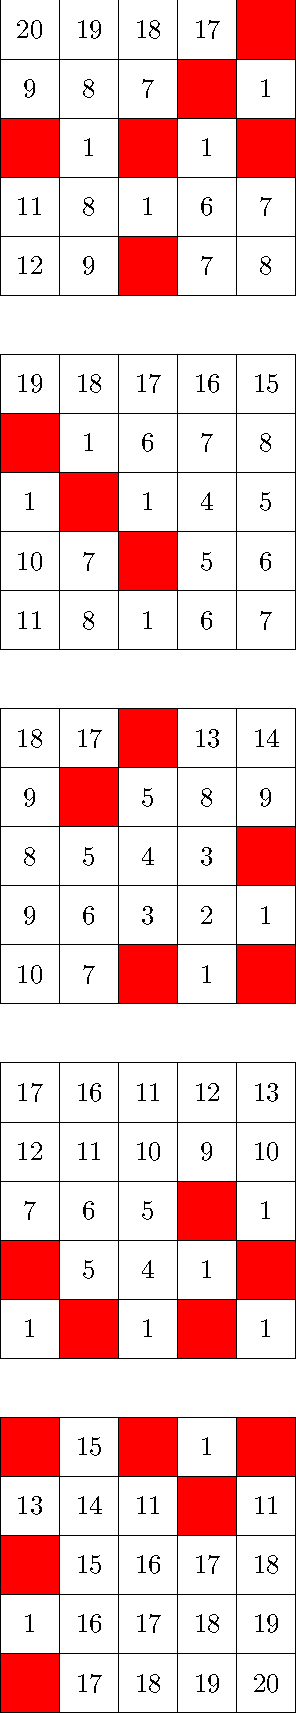
\includegraphics[width=0.2\textwidth]{figures/7/5x5x5_numbered_heatmap.pdf}
\caption{}
\label{fig:5x5x5_numbered_heatmap}
\end{figure}

% (8, 5, 5)
\begin{con}
The grid $(8,5,5)$ is perfect.
\end{con}

\begin{proof}
See figure \ref{fig:5x8x5_numbered_heatmap}.
\end{proof}

\begin{figure}[]
\centering
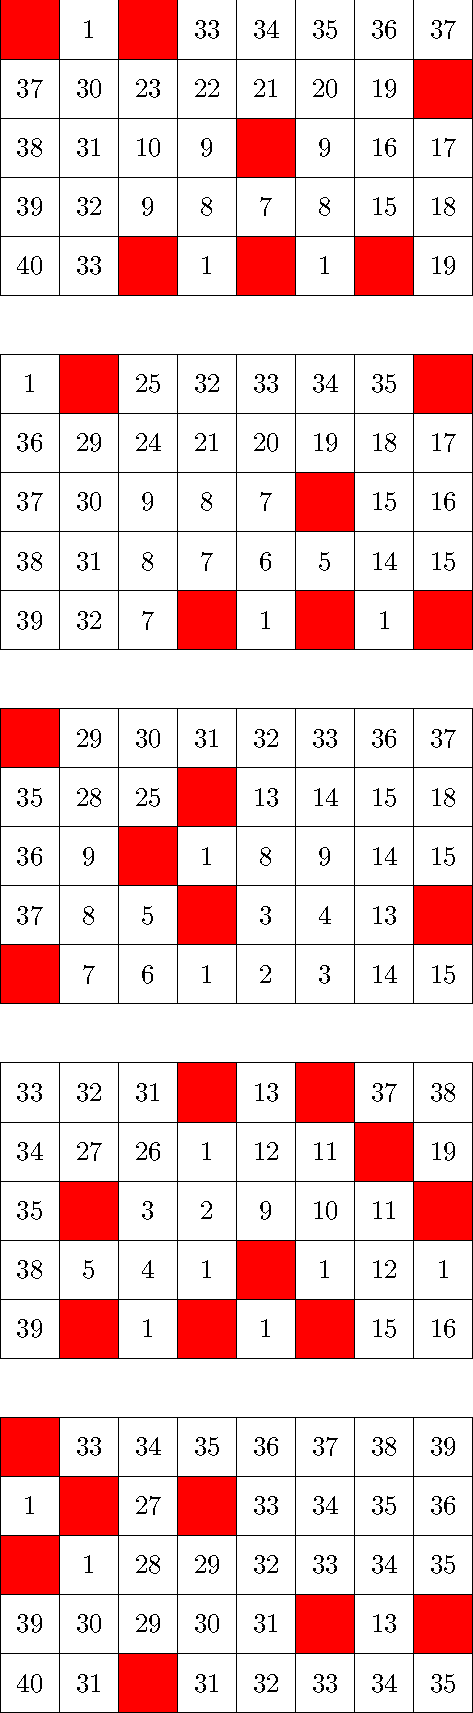
\includegraphics[width=0.2\textwidth]{figures/7/5x8x5_numbered_heatmap.pdf}
\caption{}
\label{fig:5x8x5_numbered_heatmap}
\end{figure}

% (a, 3, 3)

% (6, 3, 3)

% (6, 3, 2)

\section{Useful lemmas and observations}

We shall see that similar patterns and structures appear with some regularity in optimal sets. These structures always infect entire regions, and it will be helpful to recognize them within larger grids when they appear. 

\begin{lem}
\label{lem:forest}
Let $G = P_a \Osq P_b$ be a graph and $S \subseteq V(G)$ be a subset of the vertices of $G$. Let $G[\overline{S}]$ be the subgraph of $G$ induced by vertices not in $S$. Then $S$ is a lethal set if and only if $G[\overline{S}]$ is cycle-free, and has no paths between any two boundary vertices. 
\end{lem}

\begin{lem}
\label{lem:walls}
Let $G$ be the grid graph $(a,b,c)$ and let $A$ be a set of infected vertices in $G$. Let $H = G[\overline{A}]$ be the subgraph of $G$ induced by uninfected vertices. Let $\{F, F'\} \subseteq V(G)$ be orthogonal faces of $G$. If $H$ does not contain a path between vertices $v \in F, v' \in F'$, then $G$ percolates.
\end{lem}

\begin{proof}
We proceed by induction on $|V(H)| = abc - |A|$. If $|V(H)| = 0$, then all vertices of $G$ are infected and we are done. Suppose $|V(H)| > 0$, and consider a connected component $Y$ of $H$. By hypothesis, $Y$ does not contain a path between any two orthogonal faces of $G$. Therefore, without loss of generality, there exists a face $X = \{a\} \times \{1, \dots b\} \times \{1, \dots, c\}$ such that $V(Y) \cap X = \emptyset$. Take the largest $i$ such that $X_i = \{a\} \times \{1, \dots b\} \times \{1, \dots, c\}$ contains a vertex of $Y$. Repeat this process to obtain maximal faces $Y_j$ and $Z_k$ in the $b$ and $c$ directions, respectively. 

Observe that this construction gives a vertex $v = (i,j,k) \in V(Y)$, and planes $X_{i+1}, Y_{j+1}, Z_{k+1}$ such that $(X_{i+1} \cup Y_{j+1} \cup Z_{k+1}) \cap  V(Y) = \emptyset$. In particular, note that $(i+1,j,k), (i,j+1,k),(i,j,k+1) \in N(v)$. Since these three vertices belong to $A$ and $v \notin A$, $v$ becomes infected. Furthermore, since $|V(H) \setminus \{v\}| < |V(H)|$, the resulting graph percolates by induction. This completes the proof.
\end{proof}

\begin{cor}
\label{cor:three_walls}
Let $G$ be the grid graph $(a,b,c)$. If a set $A$ is lethal on three mutually orthogonal faces of $G$, then $A$ is lethal on $G$.
\end{cor}

\begin{proof}
Let $X, Y, Z$ be three mutually orthogonal faces of $G$. By hypothesis, $X \cup Y \cup Z \subseteq A_t$ for some time $t$. Therefore, the graph $H = G[\overline{A_t}]$ cannot contain a path between vertices on orthogonal faces of $G$. By lemma \ref{lem:walls}, $G$ percolates.
\end{proof}

\begin{cor}
\label{cor:manifold}
Let $G$ be the grid graph $(a,b,c)$ and let $A$ be a set of infected vertices of $G$. Let $\{R_1, \dots, R_k\} $ be a partition of $V(G) \setminus A$ into sub-grids $(a_1,b_1,c_1), \dots, (a_k,b_k,c_k)$ such that each $R_i$ is bounded by a lethal infection on three mutually orthogonal faces. Then $A$ is lethal on $G$.
\end{cor}

\begin{proof}
By hypothesis and corollary \ref{cor:three_walls}, $A$ is lethal on each $R_i$. Since $A \cup R_1 \cup \dots \cup R_k = V(G)$ and each $R_i$ becomes infected, $A$ must be lethal.
\end{proof}

\begin{defn}
\label{def:manifold}
Let a \emph{manifold} $M$ of the grid graph $G = (a,b,c)$ be any set of vertices $A$ satisfying the conditions of corollary \ref{cor:manifold}.
\end{defn}

\begin{defn}
\label{def:proper_unfolding}
Let a \emph{proper unfolding} of $G = (a,b,c)$ be a planar representation of the manifold of $G$. This can be thought of as a special type of folding net of $G$, such that when assembled the resulting structure satisfies the conditions of corollary \ref{cor:manifold}.
\end{defn}

\begin{cor}
\label{cor:ortho_walls}
Let $M$ be the proper unfolding of a manifold of $G = (a,b,c)$, and let $A$ be a lethal set on $M$. Then $A$ is lethal on $G$.
\end{cor}

\begin{proof}
The proof follows directly from definitions \ref{def:manifold} and \ref{def:proper_unfolding}.
\end{proof}

%\begin{cor}
%\label{cor:three_walls}
%Let $G$ be a grid assembled from sub-grids $G_1, \dots, G_k$. Let $H_1, \dots, H_k$ be sets satisfying the conditions of lemma \ref{lem:three_walls} for sub-grids $G_1, \dots, G_k$, respectively. Then $H = H_1 \cup \dots \cup H_k$ is a lethal set in $G$.
%\end{cor}

%\begin{lem}
%\label{lem:unfold}
%Let $G$ be the grid $(a,b,c)$. Let $H$ be a subgraph induced by the vertices of $G$. If the projection of $H$ in the $x$ direction gives the graph $(b,c)$, in the $y$ direction gives $(a,c)$, and in the $z$ direction gives $(a,b)$, and $H$ percolates, then $G$ percolates.
%\end{lem}

%\begin{proof}
%The projection condition guarantees that $G$ has lethal sets on three perpendicular planes. The result follows from lemma \ref{lem:three_walls}.
%\end{proof}

%We refer to the union of mutually orthogonal faces of sub-grids $G_1, \dots, G_k$ as a \emph{manifold} of $G$. Therefore, corollary \ref{cor:three_walls} says that if a set $H$ is lethal on the manifold of $G$, then $H$ is lethal in $G$. Furthermore, we define a \emph{proper unfolding} of $G$ as a planar representation of the manifold of $G$. This can be thought of as a special type of folding net of $G$, such that when assembled the resulting structure satisfies the conditions of corollary \ref{cor:three_walls}. 

%\begin{cor}
%\label{cor:unfold}
%Something about unfolding $H$ and its planar embedding. Imagine $H$ as a set of folded up pieces of paper. Let $\mathcal{N}$ be the family of unfolded nets comprising $H$. To show that $G$ percolates, it is sufficient to show that all nets $N \in \mathcal{N}$ harbor lethal infections.
%\end{cor}

\end{comment}
